\section*{Results}
\label{Results} 

Table~\ref{tab:regResults} displays the results from our model. To contrast with findings from the extant literature, we run the model in three ways. The first column tests the explanations of sanction compliance centered on target state characteristics. In the second column, we add covariates to account for a target's relationships with sender states. The final model incorporates our reciprocity measures.\footnote{In the appendix, we run a similar analysis using a set of sanctions that are imposed for security related reasons such as pursuing weapons of mass destruction. Our results for this smaller set of sanctions are consistent with what we present in Table~\ref{tab:regResults}.} 

% latex table generated in R 3.2.2 by xtable 1.7-4 package
% Sat Jul 16 11:01:02 2016
\begin{table}[ht]
\centering
{\normalsize
\begin{tabular}{lccc}
 Variable & Model 1 & Model 2 & Model 3 \\ 
  \hline
\hline
Compliance Reciprocity$_{j,t-1}$ &  &  & $0.51^{\ast\ast}$ \\ 
   &  &  & (0.1) \\ 
  Sanction Reciprocity$_{j,t-1}$ &  &  & $-0.22^{\ast\ast}$ \\ 
   &  &  & (0.06) \\ 
   \hline
Number of Senders$_{j}$ &  & $0.22^{\ast\ast}$ & $0.19^{\ast\ast}$ \\ 
   &  & (0.05) & (0.05) \\ 
  Distance$_{j}$ &  & $0.85^{\ast\ast}$ & $0.82^{\ast\ast}$ \\ 
   &  & (0.19) & (0.19) \\ 
  Trade$_{j,t-1}$ &  & -3.68 & -2.46 \\ 
   &  & (5.35) & (4.15) \\ 
  Ally$_{j,t-1}$ &  & -0.03 & 0.03 \\ 
   &  & (0.17) & (0.17) \\ 
   \hline
Polity$_{i,t-1}$ & 0.02 & $0.03^{\ast\ast}$ & 0.02 \\ 
   & (0.01) & (0.01) & (0.01) \\ 
  Ln(GDP per capita)$_{i,t-1}$ & $-0.27^{\ast\ast}$ & $-0.27^{\ast\ast}$ & $-0.22^{\ast\ast}$ \\ 
   & (0.06) & (0.06) & (0.06) \\ 
  GDP Growth$_{i,t-1}$ & 0 & 0.01 & 0 \\ 
   & (0.01) & (0.01) & (0.01) \\ 
  Population$_{i,t-1}$ & $-0.18^{\ast\ast}$ & $-0.19^{\ast\ast}$ & $-0.11^{\ast\ast}$ \\ 
   & (0.04) & (0.05) & (0.05) \\ 
  Internal Conflict$_{i,t-1}$ & 0.02 & 0.02 & 0.01 \\ 
   & (0.01) & (0.01) & (0.01) \\ 
   \hline
n & 6206 & 6183 & 6183 \\ 
  Events & 190 & 189 & 189 \\ 
  Likelihood ratio test & 54.73 (0) & 89.16 (0) & 117.21 (0) \\ 
   \hline
\hline
\end{tabular}
}
\caption{Duration model with time varying covariates estimated using Cox Proportional Hazards. Standard errors in parentheses. $^{**}$ and $^{*}$ indicate significance at $p< 0.05 $ and $p< 0.10 $, respectively.} 
\label{tab:regResults}
\end{table}


We find no support for the argument that high levels of internal stability may prompt a country to comply. Across each specification, we do find that countries with higher levels of GDP per capita take longer to comply with a sanction case, indicating that wealthier countries are able to resist complying to sanctions for lengthier durations. Additionally, like previous work in the literature, when we control for the relationships that a sanctioned state has with its senders, we find that more democratic countries are likely to take a shorter time to comply with sanctions. However, this effect becomes insignificant once we incorporate our network-related covariates. 

Since it is difficult to interpret the substantive meaning of point estimates from the hazard function in Table~\ref{tab:regResults}, we depict Kaplan-Meier estimates of survival probabilities. The y-axis in these charts represents the probability of survival, or in this case the probability that a country will not comply with a sanction, and the x-axis represents time since sanction initiation (measured in years). To depict the substantive effect of our covariates, we set up two scenarios, one in which the value for the covariate of interest is set to its minimum value, depicted in red, and another where it is set to its maximum, depicted in blue. All the other covariates are set to their median. The darker shaded area around the line represents the 90\% confidence interval and the lighter shaded area the 95\% confidence interval. Using these plots, we trace the effect of GDP per capita, in Model 3, on the probability of sanction compliance as a function of time; the results are shown in Figure~\ref{fig:monSurv}. The predicted difference in compliance probabilities between regimes with varying levels of GDP per capita, on the other hand, is quite stark. Just five years after sanction initiation, extremely poor regimes are 15\% more likely to comply than wealthier regimes. 

\begin{figure}[ht]
	\centering
	\caption{Survival probabilities over time by $Ln(GDP \; Capita)_{i,t-1}$. Red designates scenarios in which the covariate is set to its minimum value and blue where it is set to its maximum value. Darker shaded around each line represents the 90\% confidence interval and the lighter shaded area the 95\% confidence interval.}
    \resizebox{.55\textwidth}{!}{% Created by tikzDevice version 0.6.1 on 2016-06-13 09:43:08
% !TEX encoding = UTF-8 Unicode
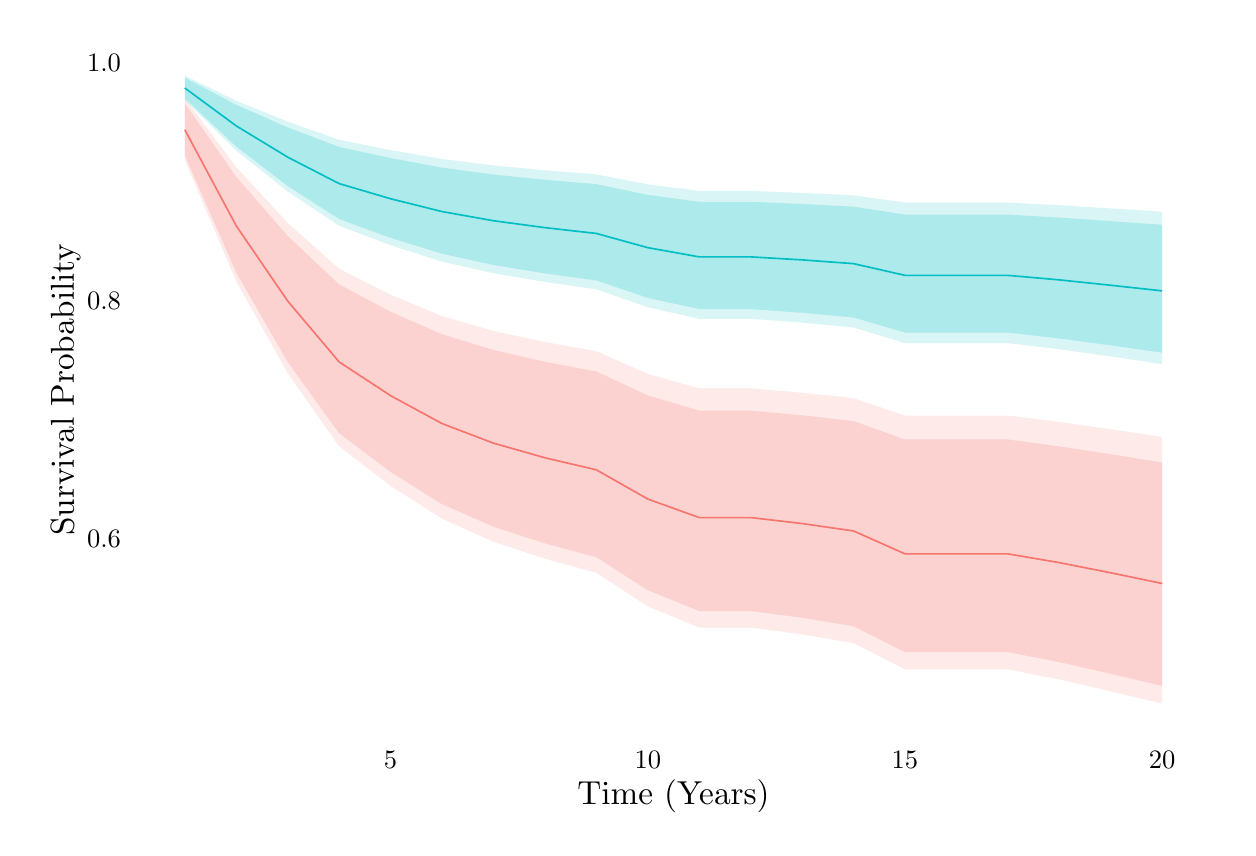
\begin{tikzpicture}[x=1pt,y=1pt]
\definecolor[named]{drawColor}{rgb}{0.00,0.00,0.00}
\definecolor[named]{fillColor}{rgb}{1.00,1.00,1.00}
\fill[color=fillColor,] (0,0) rectangle (433.62,289.08);
\begin{scope}
\path[clip] (  0.00,  0.00) rectangle (433.62,289.08);
\end{scope}
\begin{scope}
\path[clip] (  0.00,  0.00) rectangle (433.62,289.08);
\end{scope}
\begin{scope}
\path[clip] (  0.00,  0.00) rectangle (433.62,289.08);
\end{scope}
\begin{scope}
\path[clip] (  0.00,  0.00) rectangle (433.62,289.08);
\end{scope}
\begin{scope}
\path[clip] (  0.00,  0.00) rectangle (433.62,289.08);
\end{scope}
\begin{scope}
\path[clip] (  0.00,  0.00) rectangle (433.62,289.08);
\end{scope}
\begin{scope}
\path[clip] (  0.00,  0.00) rectangle (433.62,289.08);
\end{scope}
\begin{scope}
\path[clip] (  0.00,  0.00) rectangle (433.62,289.08);
\end{scope}
\begin{scope}
\path[clip] (  0.00,  0.00) rectangle (433.62,289.08);
\end{scope}
\begin{scope}
\path[clip] (  0.00,  0.00) rectangle (433.62,289.08);
\definecolor[named]{drawColor}{rgb}{1.00,1.00,1.00}
\definecolor[named]{fillColor}{rgb}{1.00,1.00,1.00}

\draw[color=drawColor,line width= 0.6pt,line cap=round,line join=round,fill=fillColor,] (  0.00,  0.00) rectangle (433.62,289.08);
\end{scope}
\begin{scope}
\path[clip] (  0.00,  0.00) rectangle (433.62,289.08);
\end{scope}
\begin{scope}
\path[clip] (  0.00,  0.00) rectangle (433.62,289.08);
\end{scope}
\begin{scope}
\path[clip] (  0.00,  0.00) rectangle (433.62,289.08);
\end{scope}
\begin{scope}
\path[clip] ( 39.13, 33.48) rectangle (427.62,283.08);
\definecolor[named]{fillColor}{rgb}{1.00,1.00,1.00}

\draw[fill=fillColor,draw opacity=0.00,] ( 39.13, 33.48) rectangle (427.62,283.08);
\definecolor[named]{drawColor}{rgb}{0.97,0.46,0.43}
\definecolor[named]{fillColor}{rgb}{0.97,0.46,0.43}

\draw[color=drawColor,line width= 0.6pt,line join=round,] ( 56.79,252.18) --
	( 75.38,217.44) --
	( 93.96,190.29) --
	(112.55,168.29) --
	(131.14,156.11) --
	(149.73,146.02) --
	(168.32,138.94) --
	(186.90,133.67) --
	(205.49,129.30) --
	(224.08,118.75) --
	(242.67,112.05) --
	(261.26,112.05) --
	(279.84,109.90) --
	(298.43,107.21) --
	(317.02, 98.94) --
	(335.61, 98.94) --
	(354.20, 98.94) --
	(372.79, 95.77) --
	(391.37, 92.09) --
	(409.96, 88.24);
\definecolor[named]{drawColor}{rgb}{0.00,0.75,0.77}
\definecolor[named]{fillColor}{rgb}{0.00,0.75,0.77}

\draw[color=drawColor,line width= 0.6pt,line join=round,] ( 56.79,267.27) --
	( 75.38,253.58) --
	( 93.96,242.29) --
	(112.55,232.73) --
	(131.14,227.26) --
	(149.73,222.63) --
	(168.32,219.31) --
	(186.90,216.82) --
	(205.49,214.72) --
	(224.08,209.58) --
	(242.67,206.25) --
	(261.26,206.25) --
	(279.84,205.17) --
	(298.43,203.81) --
	(317.02,199.58) --
	(335.61,199.58) --
	(354.20,199.58) --
	(372.79,197.94) --
	(391.37,196.00) --
	(409.96,193.97);
\definecolor[named]{fillColor}{rgb}{0.97,0.46,0.43}

\draw[fill=fillColor,fill opacity=0.15,draw opacity=0.00,] ( 56.79,263.55) --
	( 75.38,238.63) --
	( 93.96,218.49) --
	(112.55,201.93) --
	(131.14,192.55) --
	(149.73,184.85) --
	(168.32,179.47) --
	(186.90,175.46) --
	(205.49,172.13) --
	(224.08,163.94) --
	(242.67,158.74) --
	(261.26,158.74) --
	(279.84,157.15) --
	(298.43,155.17) --
	(317.02,148.92) --
	(335.61,148.92) --
	(354.20,148.92) --
	(372.79,146.59) --
	(391.37,143.97) --
	(409.96,141.17) --
	(409.96, 44.82) --
	(391.37, 49.25) --
	(372.79, 53.56) --
	(354.20, 57.21) --
	(335.61, 57.21) --
	(317.02, 57.21) --
	(298.43, 66.70) --
	(279.84, 69.85) --
	(261.26, 72.33) --
	(242.67, 72.33) --
	(224.08, 79.99) --
	(205.49, 92.11) --
	(186.90, 97.19) --
	(168.32,103.34) --
	(149.73,111.65) --
	(131.14,123.51) --
	(112.55,137.83) --
	( 93.96,164.23) --
	( 75.38,197.41) --
	( 56.79,241.12) --
	cycle;
\definecolor[named]{fillColor}{rgb}{0.00,0.75,0.77}

\draw[fill=fillColor,fill opacity=0.15,draw opacity=0.00,] ( 56.79,271.73) --
	( 75.38,262.67) --
	( 93.96,255.11) --
	(112.55,248.57) --
	(131.14,244.84) --
	(149.73,241.62) --
	(168.32,239.30) --
	(186.90,237.53) --
	(205.49,236.05) --
	(224.08,232.44) --
	(242.67,230.10) --
	(261.26,230.10) --
	(279.84,229.36) --
	(298.43,228.48) --
	(317.02,225.89) --
	(335.61,225.89) --
	(354.20,225.89) --
	(372.79,224.92) --
	(391.37,223.78) --
	(409.96,222.60) --
	(409.96,167.52) --
	(391.37,170.28) --
	(372.79,172.87) --
	(354.20,175.09) --
	(335.61,175.09) --
	(317.02,175.09) --
	(298.43,180.74) --
	(279.84,182.52) --
	(261.26,183.89) --
	(242.67,183.89) --
	(224.08,188.07) --
	(205.49,194.57) --
	(186.90,197.20) --
	(168.32,200.35) --
	(149.73,204.55) --
	(131.14,210.47) --
	(112.55,217.52) --
	( 93.96,229.88) --
	( 75.38,244.68) --
	( 56.79,262.86) --
	cycle;
\definecolor[named]{fillColor}{rgb}{0.97,0.46,0.43}

\draw[fill=fillColor,fill opacity=0.20,draw opacity=0.00,] ( 56.79,261.70) --
	( 75.38,235.14) --
	( 93.96,213.80) --
	(112.55,196.30) --
	(131.14,186.42) --
	(149.73,178.29) --
	(168.32,172.60) --
	(186.90,168.35) --
	(205.49,164.83) --
	(224.08,156.20) --
	(242.67,150.71) --
	(261.26,150.71) --
	(279.84,149.02) --
	(298.43,146.91) --
	(317.02,140.27) --
	(335.61,140.27) --
	(354.20,140.27) --
	(372.79,137.77) --
	(391.37,134.94) --
	(409.96,131.94) --
	(409.96, 51.24) --
	(391.37, 55.60) --
	(372.79, 59.83) --
	(354.20, 63.42) --
	(335.61, 63.42) --
	(317.02, 63.42) --
	(298.43, 72.76) --
	(279.84, 75.85) --
	(261.26, 78.29) --
	(242.67, 78.29) --
	(224.08, 85.82) --
	(205.49, 97.74) --
	(186.90,102.73) --
	(168.32,108.75) --
	(149.73,116.90) --
	(131.14,128.51) --
	(112.55,142.53) --
	( 93.96,168.29) --
	( 75.38,200.55) --
	( 56.79,242.88) --
	cycle;
\definecolor[named]{fillColor}{rgb}{0.00,0.75,0.77}

\draw[fill=fillColor,fill opacity=0.20,draw opacity=0.00,] ( 56.79,271.01) --
	( 75.38,261.19) --
	( 93.96,253.03) --
	(112.55,245.98) --
	(131.14,241.96) --
	(149.73,238.50) --
	(168.32,236.01) --
	(186.90,234.12) --
	(205.49,232.54) --
	(224.08,228.67) --
	(242.67,226.16) --
	(261.26,226.16) --
	(279.84,225.36) --
	(298.43,224.40) --
	(317.02,221.53) --
	(335.61,221.53) --
	(354.20,221.53) --
	(372.79,220.45) --
	(391.37,219.17) --
	(409.96,217.85) --
	(409.96,171.63) --
	(391.37,174.28) --
	(372.79,176.78) --
	(354.20,178.91) --
	(335.61,178.91) --
	(317.02,178.91) --
	(298.43,184.35) --
	(279.84,186.06) --
	(261.26,187.39) --
	(242.67,187.39) --
	(224.08,191.44) --
	(205.49,197.73) --
	(186.90,200.28) --
	(168.32,203.33) --
	(149.73,207.40) --
	(131.14,213.12) --
	(112.55,219.92) --
	( 93.96,231.85) --
	( 75.38,246.10) --
	( 56.79,263.57) --
	cycle;
\end{scope}
\begin{scope}
\path[clip] (  0.00,  0.00) rectangle (433.62,289.08);
\end{scope}
\begin{scope}
\path[clip] (  0.00,  0.00) rectangle (433.62,289.08);
\end{scope}
\begin{scope}
\path[clip] (  0.00,  0.00) rectangle (433.62,289.08);
\end{scope}
\begin{scope}
\path[clip] (  0.00,  0.00) rectangle (433.62,289.08);
\end{scope}
\begin{scope}
\path[clip] (  0.00,  0.00) rectangle (433.62,289.08);
\end{scope}
\begin{scope}
\path[clip] (  0.00,  0.00) rectangle (433.62,289.08);
\definecolor[named]{drawColor}{rgb}{0.00,0.00,0.00}

\node[color=drawColor,anchor=base east,inner sep=0pt, outer sep=0pt, scale=  0.96] at ( 33.73,101.14) {0.6%
};

\node[color=drawColor,anchor=base east,inner sep=0pt, outer sep=0pt, scale=  0.96] at ( 33.73,187.11) {0.8%
};

\node[color=drawColor,anchor=base east,inner sep=0pt, outer sep=0pt, scale=  0.96] at ( 33.73,273.08) {1.0%
};
\end{scope}
\begin{scope}
\path[clip] (  0.00,  0.00) rectangle (433.62,289.08);
\end{scope}
\begin{scope}
\path[clip] (  0.00,  0.00) rectangle (433.62,289.08);
\end{scope}
\begin{scope}
\path[clip] (  0.00,  0.00) rectangle (433.62,289.08);
\end{scope}
\begin{scope}
\path[clip] (  0.00,  0.00) rectangle (433.62,289.08);
\end{scope}
\begin{scope}
\path[clip] (  0.00,  0.00) rectangle (433.62,289.08);
\end{scope}
\begin{scope}
\path[clip] (  0.00,  0.00) rectangle (433.62,289.08);
\end{scope}
\begin{scope}
\path[clip] (  0.00,  0.00) rectangle (433.62,289.08);
\end{scope}
\begin{scope}
\path[clip] (  0.00,  0.00) rectangle (433.62,289.08);
\end{scope}
\begin{scope}
\path[clip] (  0.00,  0.00) rectangle (433.62,289.08);
\end{scope}
\begin{scope}
\path[clip] (  0.00,  0.00) rectangle (433.62,289.08);
\end{scope}
\begin{scope}
\path[clip] (  0.00,  0.00) rectangle (433.62,289.08);
\end{scope}
\begin{scope}
\path[clip] (  0.00,  0.00) rectangle (433.62,289.08);
\definecolor[named]{drawColor}{rgb}{0.00,0.00,0.00}

\node[color=drawColor,anchor=base,inner sep=0pt, outer sep=0pt, scale=  0.96] at (131.14, 21.46) {5%
};

\node[color=drawColor,anchor=base,inner sep=0pt, outer sep=0pt, scale=  0.96] at (224.08, 21.46) {10%
};

\node[color=drawColor,anchor=base,inner sep=0pt, outer sep=0pt, scale=  0.96] at (317.02, 21.46) {15%
};

\node[color=drawColor,anchor=base,inner sep=0pt, outer sep=0pt, scale=  0.96] at (409.96, 21.46) {20%
};
\end{scope}
\begin{scope}
\path[clip] (  0.00,  0.00) rectangle (433.62,289.08);
\end{scope}
\begin{scope}
\path[clip] (  0.00,  0.00) rectangle (433.62,289.08);
\end{scope}
\begin{scope}
\path[clip] (  0.00,  0.00) rectangle (433.62,289.08);
\end{scope}
\begin{scope}
\path[clip] (  0.00,  0.00) rectangle (433.62,289.08);
\definecolor[named]{drawColor}{rgb}{0.00,0.00,0.00}

\node[color=drawColor,anchor=base,inner sep=0pt, outer sep=0pt, scale=  1.20] at (233.37,  8.40) {Time (Years)%
};
\end{scope}
\begin{scope}
\path[clip] (  0.00,  0.00) rectangle (433.62,289.08);
\end{scope}
\begin{scope}
\path[clip] (  0.00,  0.00) rectangle (433.62,289.08);
\definecolor[named]{drawColor}{rgb}{0.00,0.00,0.00}

\node[rotate= 90.00,color=drawColor,anchor=base,inner sep=0pt, outer sep=0pt, scale=  1.20] at ( 16.66,158.28) {Survival Probability%
};
\end{scope}
\begin{scope}
\path[clip] (  0.00,  0.00) rectangle (433.62,289.08);
\end{scope}
\begin{scope}
\path[clip] (  0.00,  0.00) rectangle (433.62,289.08);
\end{scope}
\begin{scope}
\path[clip] (  0.00,  0.00) rectangle (433.62,289.08);
\end{scope}
\begin{scope}
\path[clip] (  0.00,  0.00) rectangle (433.62,289.08);
\end{scope}
\end{tikzpicture}
}	
	\label{fig:monSurv}
\end{figure}

We also find strong support for the argument that states are more likely to comply with sanctions involving multiple actors, and the effect of this variable remains consistent even after controlling for our network level covariates in Model 3. Using Figure~\ref{fig:nosSurv} we can quickly see that there is a stark difference in the likelihood of non-compliance between a sanction case involving single and multiple senders. After just five years the probability of non-compliance drops to approximately 60\%, whereas a sanction from a single sender by that time still has an 85\% chance of non-compliance. Unlike the extant literature, we do not find strong evidence for the ability of trading partners to obtain quick and successful resolutions to sanction cases. States are also not likely to comply more quickly to sanctions sent by allies, and are actually less likely to comply with sanctions sent from neighbors. 

\begin{figure}[ht]
	\centering
	\caption{Survival probabilities over time by the number of senders in a sanction case.}
	\resizebox{0.55\textwidth}{!}{% Created by tikzDevice version 0.6.1 on 2016-07-16 10:57:14
% !TEX encoding = UTF-8 Unicode
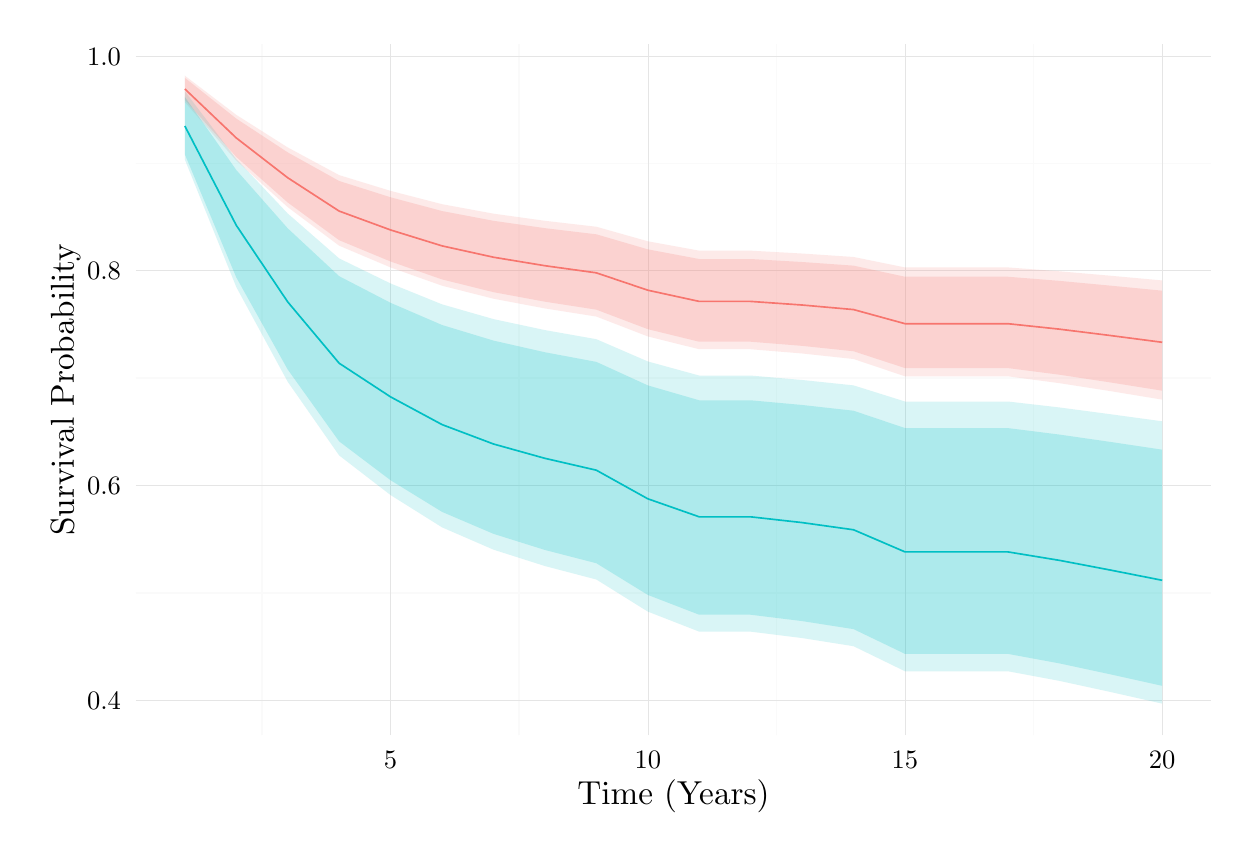
\begin{tikzpicture}[x=1pt,y=1pt]
\definecolor[named]{drawColor}{rgb}{0.00,0.00,0.00}
\definecolor[named]{fillColor}{rgb}{1.00,1.00,1.00}
\fill[color=fillColor,] (0,0) rectangle (433.62,289.08);
\begin{scope}
\path[clip] (  0.00,  0.00) rectangle (433.62,289.08);
\definecolor[named]{fillColor}{rgb}{0.00,0.00,0.00}
\end{scope}
\begin{scope}
\path[clip] (  0.00,  0.00) rectangle (433.62,289.08);
\definecolor[named]{fillColor}{rgb}{0.00,0.00,0.00}
\end{scope}
\begin{scope}
\path[clip] (  0.00,  0.00) rectangle (433.62,289.08);
\definecolor[named]{fillColor}{rgb}{0.00,0.00,0.00}
\end{scope}
\begin{scope}
\path[clip] (  0.00,  0.00) rectangle (433.62,289.08);
\definecolor[named]{fillColor}{rgb}{0.00,0.00,0.00}
\end{scope}
\begin{scope}
\path[clip] (  0.00,  0.00) rectangle (433.62,289.08);
\definecolor[named]{fillColor}{rgb}{0.00,0.00,0.00}
\end{scope}
\begin{scope}
\path[clip] (  0.00,  0.00) rectangle (433.62,289.08);
\definecolor[named]{fillColor}{rgb}{0.00,0.00,0.00}
\end{scope}
\begin{scope}
\path[clip] (  0.00,  0.00) rectangle (433.62,289.08);
\definecolor[named]{fillColor}{rgb}{0.00,0.00,0.00}
\end{scope}
\begin{scope}
\path[clip] (  0.00,  0.00) rectangle (433.62,289.08);
\definecolor[named]{fillColor}{rgb}{0.00,0.00,0.00}
\end{scope}
\begin{scope}
\path[clip] (  0.00,  0.00) rectangle (433.62,289.08);
\definecolor[named]{fillColor}{rgb}{0.00,0.00,0.00}
\end{scope}
\begin{scope}
\path[clip] (  0.00,  0.00) rectangle (433.62,289.08);
\definecolor[named]{fillColor}{rgb}{0.00,0.00,0.00}
\definecolor[named]{drawColor}{rgb}{1.00,1.00,1.00}
\definecolor[named]{fillColor}{rgb}{1.00,1.00,1.00}

\draw[color=drawColor,line width= 0.6pt,line cap=round,line join=round,fill=fillColor,] (  0.00,  0.00) rectangle (433.62,289.08);
\end{scope}
\begin{scope}
\path[clip] (  0.00,  0.00) rectangle (433.62,289.08);
\definecolor[named]{fillColor}{rgb}{0.00,0.00,0.00}
\end{scope}
\begin{scope}
\path[clip] (  0.00,  0.00) rectangle (433.62,289.08);
\definecolor[named]{fillColor}{rgb}{0.00,0.00,0.00}
\end{scope}
\begin{scope}
\path[clip] (  0.00,  0.00) rectangle (433.62,289.08);
\definecolor[named]{fillColor}{rgb}{0.00,0.00,0.00}
\end{scope}
\begin{scope}
\path[clip] ( 39.13, 33.48) rectangle (427.62,283.08);
\definecolor[named]{fillColor}{rgb}{0.00,0.00,0.00}
\definecolor[named]{fillColor}{rgb}{1.00,1.00,1.00}

\draw[fill=fillColor,draw opacity=0.00,] ( 39.13, 33.48) rectangle (427.62,283.08);
\definecolor[named]{drawColor}{rgb}{0.98,0.98,0.98}

\draw[color=drawColor,line width= 0.6pt,line join=round,fill opacity=0.00,] ( 39.13, 84.80) --
	(427.62, 84.80);

\draw[color=drawColor,line width= 0.6pt,line join=round,fill opacity=0.00,] ( 39.13,162.43) --
	(427.62,162.43);

\draw[color=drawColor,line width= 0.6pt,line join=round,fill opacity=0.00,] ( 39.13,240.05) --
	(427.62,240.05);

\draw[color=drawColor,line width= 0.6pt,line join=round,fill opacity=0.00,] ( 84.67, 33.48) --
	( 84.67,283.08);

\draw[color=drawColor,line width= 0.6pt,line join=round,fill opacity=0.00,] (177.61, 33.48) --
	(177.61,283.08);

\draw[color=drawColor,line width= 0.6pt,line join=round,fill opacity=0.00,] (270.55, 33.48) --
	(270.55,283.08);

\draw[color=drawColor,line width= 0.6pt,line join=round,fill opacity=0.00,] (363.49, 33.48) --
	(363.49,283.08);
\definecolor[named]{drawColor}{rgb}{0.90,0.90,0.90}

\draw[color=drawColor,line width= 0.2pt,line join=round,fill opacity=0.00,] ( 39.13, 45.99) --
	(427.62, 45.99);

\draw[color=drawColor,line width= 0.2pt,line join=round,fill opacity=0.00,] ( 39.13,123.61) --
	(427.62,123.61);

\draw[color=drawColor,line width= 0.2pt,line join=round,fill opacity=0.00,] ( 39.13,201.24) --
	(427.62,201.24);

\draw[color=drawColor,line width= 0.2pt,line join=round,fill opacity=0.00,] ( 39.13,278.86) --
	(427.62,278.86);

\draw[color=drawColor,line width= 0.2pt,line join=round,fill opacity=0.00,] (131.14, 33.48) --
	(131.14,283.08);

\draw[color=drawColor,line width= 0.2pt,line join=round,fill opacity=0.00,] (224.08, 33.48) --
	(224.08,283.08);

\draw[color=drawColor,line width= 0.2pt,line join=round,fill opacity=0.00,] (317.02, 33.48) --
	(317.02,283.08);

\draw[color=drawColor,line width= 0.2pt,line join=round,fill opacity=0.00,] (409.96, 33.48) --
	(409.96,283.08);
\definecolor[named]{drawColor}{rgb}{0.97,0.46,0.43}
\definecolor[named]{fillColor}{rgb}{0.97,0.46,0.43}

\draw[color=drawColor,line width= 0.6pt,line join=round,] ( 56.79,266.93) --
	( 75.38,249.23) --
	( 93.96,234.85) --
	(112.55,222.80) --
	(131.14,215.98) --
	(149.73,210.23) --
	(168.32,206.13) --
	(186.90,203.06) --
	(205.49,200.49) --
	(224.08,194.21) --
	(242.67,190.16) --
	(261.26,190.16) --
	(279.84,188.86) --
	(298.43,187.21) --
	(317.02,182.11) --
	(335.61,182.11) --
	(354.20,182.11) --
	(372.79,180.14) --
	(391.37,177.82) --
	(409.96,175.39);
\definecolor[named]{drawColor}{rgb}{0.00,0.75,0.77}
\definecolor[named]{fillColor}{rgb}{0.00,0.75,0.77}

\draw[color=drawColor,line width= 0.6pt,line join=round,] ( 56.79,253.55) --
	( 75.38,217.66) --
	( 93.96,189.99) --
	(112.55,167.83) --
	(131.14,155.66) --
	(149.73,145.65) --
	(168.32,138.64) --
	(186.90,133.46) --
	(205.49,129.17) --
	(224.08,118.84) --
	(242.67,112.32) --
	(261.26,112.32) --
	(279.84,110.24) --
	(298.43,107.64) --
	(317.02, 99.65) --
	(335.61, 99.65) --
	(354.20, 99.65) --
	(372.79, 96.60) --
	(391.37, 93.06) --
	(409.96, 89.39);
\definecolor[named]{fillColor}{rgb}{0.97,0.46,0.43}

\draw[fill=fillColor,fill opacity=0.15,draw opacity=0.00,] ( 56.79,271.73) --
	( 75.38,257.57) --
	( 93.96,245.80) --
	(112.55,235.80) --
	(131.14,230.10) --
	(149.73,225.29) --
	(168.32,221.87) --
	(186.90,219.29) --
	(205.49,217.14) --
	(224.08,211.89) --
	(242.67,208.50) --
	(261.26,208.50) --
	(279.84,207.46) --
	(298.43,206.22) --
	(317.02,202.44) --
	(335.61,202.44) --
	(354.20,202.44) --
	(372.79,201.05) --
	(391.37,199.43) --
	(409.96,197.74) --
	(409.96,154.67) --
	(391.37,157.73) --
	(372.79,160.63) --
	(354.20,163.10) --
	(335.61,163.10) --
	(317.02,163.10) --
	(298.43,169.35) --
	(279.84,171.35) --
	(261.26,172.88) --
	(242.67,172.88) --
	(224.08,177.51) --
	(205.49,184.69) --
	(186.90,187.63) --
	(168.32,191.14) --
	(149.73,195.84) --
	(131.14,202.44) --
	(112.55,210.30) --
	( 93.96,224.23) --
	( 75.38,241.07) --
	( 56.79,262.19) --
	cycle;
\definecolor[named]{fillColor}{rgb}{0.00,0.75,0.77}

\draw[fill=fillColor,fill opacity=0.15,draw opacity=0.00,] ( 56.79,266.11) --
	( 75.38,241.61) --
	( 93.96,221.94) --
	(112.55,205.70) --
	(131.14,196.64) --
	(149.73,189.10) --
	(168.32,183.77) --
	(186.90,179.80) --
	(205.49,176.51) --
	(224.08,168.47) --
	(242.67,163.37) --
	(261.26,163.37) --
	(279.84,161.77) --
	(298.43,159.82) --
	(317.02,153.99) --
	(335.61,153.99) --
	(354.20,153.99) --
	(372.79,151.85) --
	(391.37,149.38) --
	(409.96,146.84) --
	(409.96, 44.82) --
	(391.37, 49.01) --
	(372.79, 53.05) --
	(354.20, 56.52) --
	(335.61, 56.52) --
	(317.02, 56.52) --
	(298.43, 65.57) --
	(279.84, 68.52) --
	(261.26, 70.83) --
	(242.67, 70.83) --
	(224.08, 78.08) --
	(205.49, 89.67) --
	(186.90, 94.54) --
	(168.32,100.46) --
	(149.73,108.52) --
	(131.14,120.18) --
	(112.55,134.51) --
	( 93.96,161.13) --
	( 75.38,195.36) --
	( 56.79,241.41) --
	cycle;
\definecolor[named]{fillColor}{rgb}{0.97,0.46,0.43}

\draw[fill=fillColor,fill opacity=0.20,draw opacity=0.00,] ( 56.79,270.96) --
	( 75.38,256.22) --
	( 93.96,244.02) --
	(112.55,233.68) --
	(131.14,227.79) --
	(149.73,222.82) --
	(168.32,219.29) --
	(186.90,216.63) --
	(205.49,214.41) --
	(224.08,208.98) --
	(242.67,205.48) --
	(261.26,205.48) --
	(279.84,204.40) --
	(298.43,203.09) --
	(317.02,199.08) --
	(335.61,199.08) --
	(354.20,199.08) --
	(372.79,197.59) --
	(391.37,195.85) --
	(409.96,194.04) --
	(409.96,157.90) --
	(391.37,160.86) --
	(372.79,163.68) --
	(354.20,166.07) --
	(335.61,166.07) --
	(317.02,166.07) --
	(298.43,172.15) --
	(279.84,174.10) --
	(261.26,175.59) --
	(242.67,175.59) --
	(224.08,180.13) --
	(205.49,187.18) --
	(186.90,190.06) --
	(168.32,193.50) --
	(149.73,198.11) --
	(131.14,204.58) --
	(112.55,212.28) --
	( 93.96,225.91) --
	( 75.38,242.37) --
	( 56.79,262.95) --
	cycle;
\definecolor[named]{fillColor}{rgb}{0.00,0.75,0.77}

\draw[fill=fillColor,fill opacity=0.20,draw opacity=0.00,] ( 56.79,264.06) --
	( 75.38,237.64) --
	( 93.96,216.58) --
	(112.55,199.28) --
	(131.14,189.65) --
	(149.73,181.64) --
	(168.32,176.00) --
	(186.90,171.79) --
	(205.49,168.31) --
	(224.08,159.82) --
	(242.67,154.43) --
	(261.26,154.43) --
	(279.84,152.74) --
	(298.43,150.66) --
	(317.02,144.39) --
	(335.61,144.39) --
	(354.20,144.39) --
	(372.79,142.05) --
	(391.37,139.37) --
	(409.96,136.59) --
	(409.96, 51.25) --
	(391.37, 55.38) --
	(372.79, 59.37) --
	(354.20, 62.80) --
	(335.61, 62.80) --
	(317.02, 62.80) --
	(298.43, 71.74) --
	(279.84, 74.65) --
	(261.26, 76.94) --
	(242.67, 76.94) --
	(224.08, 84.11) --
	(205.49, 95.55) --
	(186.90,100.35) --
	(168.32,106.18) --
	(149.73,114.11) --
	(131.14,125.54) --
	(112.55,139.58) --
	( 93.96,165.57) --
	( 75.38,198.84) --
	( 56.79,243.33) --
	cycle;
\end{scope}
\begin{scope}
\path[clip] (  0.00,  0.00) rectangle (433.62,289.08);
\definecolor[named]{fillColor}{rgb}{0.00,0.00,0.00}
\end{scope}
\begin{scope}
\path[clip] (  0.00,  0.00) rectangle (433.62,289.08);
\definecolor[named]{fillColor}{rgb}{0.00,0.00,0.00}
\end{scope}
\begin{scope}
\path[clip] (  0.00,  0.00) rectangle (433.62,289.08);
\definecolor[named]{fillColor}{rgb}{0.00,0.00,0.00}
\end{scope}
\begin{scope}
\path[clip] (  0.00,  0.00) rectangle (433.62,289.08);
\definecolor[named]{fillColor}{rgb}{0.00,0.00,0.00}
\end{scope}
\begin{scope}
\path[clip] (  0.00,  0.00) rectangle (433.62,289.08);
\definecolor[named]{fillColor}{rgb}{0.00,0.00,0.00}
\end{scope}
\begin{scope}
\path[clip] (  0.00,  0.00) rectangle (433.62,289.08);
\definecolor[named]{fillColor}{rgb}{0.00,0.00,0.00}
\definecolor[named]{drawColor}{rgb}{0.00,0.00,0.00}

\node[color=drawColor,anchor=base east,inner sep=0pt, outer sep=0pt, scale=  0.96] at ( 33.73, 42.68) {0.4%
};

\node[color=drawColor,anchor=base east,inner sep=0pt, outer sep=0pt, scale=  0.96] at ( 33.73,120.31) {0.6%
};

\node[color=drawColor,anchor=base east,inner sep=0pt, outer sep=0pt, scale=  0.96] at ( 33.73,197.93) {0.8%
};

\node[color=drawColor,anchor=base east,inner sep=0pt, outer sep=0pt, scale=  0.96] at ( 33.73,275.56) {1.0%
};
\end{scope}
\begin{scope}
\path[clip] (  0.00,  0.00) rectangle (433.62,289.08);
\definecolor[named]{fillColor}{rgb}{0.00,0.00,0.00}
\end{scope}
\begin{scope}
\path[clip] (  0.00,  0.00) rectangle (433.62,289.08);
\definecolor[named]{fillColor}{rgb}{0.00,0.00,0.00}
\end{scope}
\begin{scope}
\path[clip] (  0.00,  0.00) rectangle (433.62,289.08);
\definecolor[named]{fillColor}{rgb}{0.00,0.00,0.00}
\end{scope}
\begin{scope}
\path[clip] (  0.00,  0.00) rectangle (433.62,289.08);
\definecolor[named]{fillColor}{rgb}{0.00,0.00,0.00}
\end{scope}
\begin{scope}
\path[clip] (  0.00,  0.00) rectangle (433.62,289.08);
\definecolor[named]{fillColor}{rgb}{0.00,0.00,0.00}
\end{scope}
\begin{scope}
\path[clip] (  0.00,  0.00) rectangle (433.62,289.08);
\definecolor[named]{fillColor}{rgb}{0.00,0.00,0.00}
\end{scope}
\begin{scope}
\path[clip] (  0.00,  0.00) rectangle (433.62,289.08);
\definecolor[named]{fillColor}{rgb}{0.00,0.00,0.00}
\end{scope}
\begin{scope}
\path[clip] (  0.00,  0.00) rectangle (433.62,289.08);
\definecolor[named]{fillColor}{rgb}{0.00,0.00,0.00}
\end{scope}
\begin{scope}
\path[clip] (  0.00,  0.00) rectangle (433.62,289.08);
\definecolor[named]{fillColor}{rgb}{0.00,0.00,0.00}
\end{scope}
\begin{scope}
\path[clip] (  0.00,  0.00) rectangle (433.62,289.08);
\definecolor[named]{fillColor}{rgb}{0.00,0.00,0.00}
\end{scope}
\begin{scope}
\path[clip] (  0.00,  0.00) rectangle (433.62,289.08);
\definecolor[named]{fillColor}{rgb}{0.00,0.00,0.00}
\end{scope}
\begin{scope}
\path[clip] (  0.00,  0.00) rectangle (433.62,289.08);
\definecolor[named]{fillColor}{rgb}{0.00,0.00,0.00}
\definecolor[named]{drawColor}{rgb}{0.00,0.00,0.00}

\node[color=drawColor,anchor=base,inner sep=0pt, outer sep=0pt, scale=  0.96] at (131.14, 21.46) {5%
};

\node[color=drawColor,anchor=base,inner sep=0pt, outer sep=0pt, scale=  0.96] at (224.08, 21.46) {10%
};

\node[color=drawColor,anchor=base,inner sep=0pt, outer sep=0pt, scale=  0.96] at (317.02, 21.46) {15%
};

\node[color=drawColor,anchor=base,inner sep=0pt, outer sep=0pt, scale=  0.96] at (409.96, 21.46) {20%
};
\end{scope}
\begin{scope}
\path[clip] (  0.00,  0.00) rectangle (433.62,289.08);
\definecolor[named]{fillColor}{rgb}{0.00,0.00,0.00}
\end{scope}
\begin{scope}
\path[clip] (  0.00,  0.00) rectangle (433.62,289.08);
\definecolor[named]{fillColor}{rgb}{0.00,0.00,0.00}
\end{scope}
\begin{scope}
\path[clip] (  0.00,  0.00) rectangle (433.62,289.08);
\definecolor[named]{fillColor}{rgb}{0.00,0.00,0.00}
\end{scope}
\begin{scope}
\path[clip] (  0.00,  0.00) rectangle (433.62,289.08);
\definecolor[named]{fillColor}{rgb}{0.00,0.00,0.00}
\definecolor[named]{drawColor}{rgb}{0.00,0.00,0.00}

\node[color=drawColor,anchor=base,inner sep=0pt, outer sep=0pt, scale=  1.20] at (233.37,  8.40) {Time (Years)%
};
\end{scope}
\begin{scope}
\path[clip] (  0.00,  0.00) rectangle (433.62,289.08);
\definecolor[named]{fillColor}{rgb}{0.00,0.00,0.00}
\end{scope}
\begin{scope}
\path[clip] (  0.00,  0.00) rectangle (433.62,289.08);
\definecolor[named]{fillColor}{rgb}{0.00,0.00,0.00}
\definecolor[named]{drawColor}{rgb}{0.00,0.00,0.00}

\node[rotate= 90.00,color=drawColor,anchor=base,inner sep=0pt, outer sep=0pt, scale=  1.20] at ( 16.66,158.28) {Survival Probability%
};
\end{scope}
\begin{scope}
\path[clip] (  0.00,  0.00) rectangle (433.62,289.08);
\definecolor[named]{fillColor}{rgb}{0.00,0.00,0.00}
\end{scope}
\begin{scope}
\path[clip] (  0.00,  0.00) rectangle (433.62,289.08);
\definecolor[named]{fillColor}{rgb}{0.00,0.00,0.00}
\end{scope}
\begin{scope}
\path[clip] (  0.00,  0.00) rectangle (433.62,289.08);
\definecolor[named]{fillColor}{rgb}{0.00,0.00,0.00}
\end{scope}
\begin{scope}
\path[clip] (  0.00,  0.00) rectangle (433.62,289.08);
\definecolor[named]{fillColor}{rgb}{0.00,0.00,0.00}
\end{scope}
\end{tikzpicture}
}
	\label{fig:nosSurv}
\end{figure}

Our key hypothesis relates to the effect of compliance and sanction reciprocity. We incorporate these variables in the last column of Table~\ref{tab:regResults} and here we find that target states comply much more quickly to sanctions sent from countries with whom they have a strong history of reciprocal compliance relative to others in the network. On the left side of Figure~\ref{fig:surv3}, we can see that after just five years, the probability of non-compliance in sanction cases where target and sender states have a history of reciprocal compliance is approximately 60\%, compared to about 90\% when this history does not exist between senders and receivers. 

\begin{figure}[ht]
	\centering
	\caption{Survival probabilities reflecting over time by network level covariates.}
	\begin{tabular}{cc}

	\subfloat[Subfigure 1][Compliance Reciprocity]{
		\resizebox{.45\textwidth}{!}{% Created by tikzDevice version 0.6.1 on 2016-06-13 09:43:08
% !TEX encoding = UTF-8 Unicode
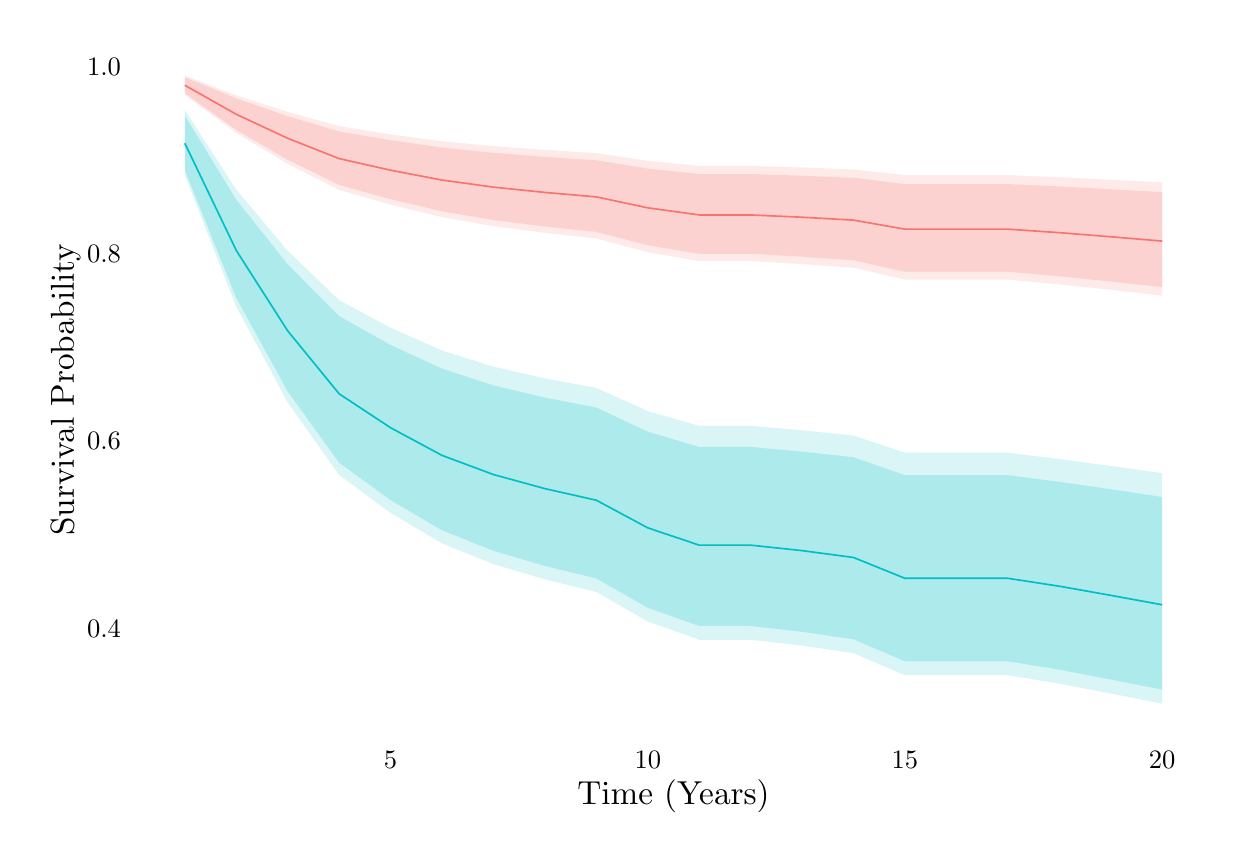
\begin{tikzpicture}[x=1pt,y=1pt]
\definecolor[named]{drawColor}{rgb}{0.00,0.00,0.00}
\definecolor[named]{fillColor}{rgb}{1.00,1.00,1.00}
\fill[color=fillColor,] (0,0) rectangle (433.62,289.08);
\begin{scope}
\path[clip] (  0.00,  0.00) rectangle (433.62,289.08);
\end{scope}
\begin{scope}
\path[clip] (  0.00,  0.00) rectangle (433.62,289.08);
\end{scope}
\begin{scope}
\path[clip] (  0.00,  0.00) rectangle (433.62,289.08);
\end{scope}
\begin{scope}
\path[clip] (  0.00,  0.00) rectangle (433.62,289.08);
\end{scope}
\begin{scope}
\path[clip] (  0.00,  0.00) rectangle (433.62,289.08);
\end{scope}
\begin{scope}
\path[clip] (  0.00,  0.00) rectangle (433.62,289.08);
\end{scope}
\begin{scope}
\path[clip] (  0.00,  0.00) rectangle (433.62,289.08);
\end{scope}
\begin{scope}
\path[clip] (  0.00,  0.00) rectangle (433.62,289.08);
\end{scope}
\begin{scope}
\path[clip] (  0.00,  0.00) rectangle (433.62,289.08);
\end{scope}
\begin{scope}
\path[clip] (  0.00,  0.00) rectangle (433.62,289.08);
\definecolor[named]{drawColor}{rgb}{1.00,1.00,1.00}
\definecolor[named]{fillColor}{rgb}{1.00,1.00,1.00}

\draw[color=drawColor,line width= 0.6pt,line cap=round,line join=round,fill=fillColor,] (  0.00,  0.00) rectangle (433.62,289.08);
\end{scope}
\begin{scope}
\path[clip] (  0.00,  0.00) rectangle (433.62,289.08);
\end{scope}
\begin{scope}
\path[clip] (  0.00,  0.00) rectangle (433.62,289.08);
\end{scope}
\begin{scope}
\path[clip] (  0.00,  0.00) rectangle (433.62,289.08);
\end{scope}
\begin{scope}
\path[clip] ( 39.13, 33.48) rectangle (427.62,283.08);
\definecolor[named]{fillColor}{rgb}{1.00,1.00,1.00}

\draw[fill=fillColor,draw opacity=0.00,] ( 39.13, 33.48) rectangle (427.62,283.08);
\definecolor[named]{drawColor}{rgb}{0.97,0.46,0.43}
\definecolor[named]{fillColor}{rgb}{0.97,0.46,0.43}

\draw[color=drawColor,line width= 0.6pt,line join=round,] ( 56.79,268.27) --
	( 75.38,257.77) --
	( 93.96,249.11) --
	(112.55,241.77) --
	(131.14,237.57) --
	(149.73,234.01) --
	(168.32,231.46) --
	(186.90,229.54) --
	(205.49,227.93) --
	(224.08,223.97) --
	(242.67,221.41) --
	(261.26,221.41) --
	(279.84,220.58) --
	(298.43,219.53) --
	(317.02,216.27) --
	(335.61,216.27) --
	(354.20,216.27) --
	(372.79,215.01) --
	(391.37,213.52) --
	(409.96,211.96);
\definecolor[named]{drawColor}{rgb}{0.00,0.75,0.77}
\definecolor[named]{fillColor}{rgb}{0.00,0.75,0.77}

\draw[color=drawColor,line width= 0.6pt,line join=round,] ( 56.79,247.29) --
	( 75.38,208.58) --
	( 93.96,179.52) --
	(112.55,156.77) --
	(131.14,144.51) --
	(149.73,134.52) --
	(168.32,127.60) --
	(186.90,122.51) --
	(205.49,118.32) --
	(224.08,108.33) --
	(242.67,102.09) --
	(261.26,102.09) --
	(279.84,100.11) --
	(298.43, 97.63) --
	(317.02, 90.10) --
	(335.61, 90.10) --
	(354.20, 90.10) --
	(372.79, 87.25) --
	(391.37, 83.95) --
	(409.96, 80.54);
\definecolor[named]{fillColor}{rgb}{0.97,0.46,0.43}

\draw[fill=fillColor,fill opacity=0.15,draw opacity=0.00,] ( 56.79,271.73) --
	( 75.38,264.63) --
	( 93.96,258.64) --
	(112.55,253.47) --
	(131.14,250.53) --
	(149.73,248.03) --
	(168.32,246.26) --
	(186.90,244.89) --
	(205.49,243.75) --
	(224.08,240.94) --
	(242.67,239.12) --
	(261.26,239.12) --
	(279.84,238.55) --
	(298.43,237.85) --
	(317.02,235.79) --
	(335.61,235.79) --
	(354.20,235.79) --
	(372.79,235.02) --
	(391.37,234.11) --
	(409.96,233.15) --
	(409.96,192.27) --
	(391.37,194.36) --
	(372.79,196.34) --
	(354.20,198.03) --
	(335.61,198.03) --
	(317.02,198.03) --
	(298.43,202.33) --
	(279.84,203.68) --
	(261.26,204.74) --
	(242.67,204.74) --
	(224.08,207.95) --
	(205.49,212.92) --
	(186.90,214.95) --
	(168.32,217.37) --
	(149.73,220.62) --
	(131.14,225.14) --
	(112.55,230.50) --
	( 93.96,239.87) --
	( 75.38,251.05) --
	( 56.79,264.84) --
	cycle;
\definecolor[named]{fillColor}{rgb}{0.00,0.75,0.77}

\draw[fill=fillColor,fill opacity=0.15,draw opacity=0.00,] ( 56.79,259.26) --
	( 75.38,230.54) --
	( 93.96,208.42) --
	(112.55,190.63) --
	(131.14,180.62) --
	(149.73,172.42) --
	(168.32,166.56) --
	(186.90,162.34) --
	(205.49,158.89) --
	(224.08,150.48) --
	(242.67,145.20) --
	(261.26,145.20) --
	(279.84,143.59) --
	(298.43,141.67) --
	(317.02,135.48) --
	(335.61,135.48) --
	(354.20,135.48) --
	(372.79,133.20) --
	(391.37,130.70) --
	(409.96,128.06) --
	(409.96, 44.82) --
	(391.37, 48.47) --
	(372.79, 52.05) --
	(354.20, 55.08) --
	(335.61, 55.08) --
	(317.02, 55.08) --
	(298.43, 63.06) --
	(279.84, 65.78) --
	(261.26, 67.90) --
	(242.67, 67.90) --
	(224.08, 74.50) --
	(205.49, 85.17) --
	(186.90, 89.71) --
	(168.32, 95.24) --
	(149.73,102.72) --
	(131.14,113.74) --
	(112.55,127.43) --
	( 93.96,153.70) --
	( 75.38,188.26) --
	( 56.79,235.76) --
	cycle;
\definecolor[named]{fillColor}{rgb}{0.97,0.46,0.43}

\draw[fill=fillColor,fill opacity=0.20,draw opacity=0.00,] ( 56.79,271.18) --
	( 75.38,263.52) --
	( 93.96,257.09) --
	(112.55,251.56) --
	(131.14,248.41) --
	(149.73,245.73) --
	(168.32,243.83) --
	(186.90,242.37) --
	(205.49,241.15) --
	(224.08,238.15) --
	(242.67,236.20) --
	(261.26,236.20) --
	(279.84,235.59) --
	(298.43,234.83) --
	(317.02,232.57) --
	(335.61,232.57) --
	(354.20,232.57) --
	(372.79,231.71) --
	(391.37,230.70) --
	(409.96,229.64) --
	(409.96,195.34) --
	(391.37,197.35) --
	(372.79,199.25) --
	(354.20,200.88) --
	(335.61,200.88) --
	(317.02,200.88) --
	(298.43,205.02) --
	(279.84,206.33) --
	(261.26,207.35) --
	(242.67,207.35) --
	(224.08,210.46) --
	(205.49,215.28) --
	(186.90,217.24) --
	(168.32,219.58) --
	(149.73,222.73) --
	(131.14,227.10) --
	(112.55,232.28) --
	( 93.96,241.34) --
	( 75.38,252.12) --
	( 56.79,265.39) --
	cycle;
\definecolor[named]{fillColor}{rgb}{0.00,0.75,0.77}

\draw[fill=fillColor,fill opacity=0.20,draw opacity=0.00,] ( 56.79,257.31) --
	( 75.38,226.89) --
	( 93.96,203.55) --
	(112.55,184.86) --
	(131.14,174.41) --
	(149.73,165.87) --
	(168.32,159.80) --
	(186.90,155.40) --
	(205.49,151.80) --
	(224.08,143.07) --
	(242.67,137.58) --
	(261.26,137.58) --
	(279.84,135.89) --
	(298.43,133.85) --
	(317.02,127.37) --
	(335.61,127.37) --
	(354.20,127.37) --
	(372.79,124.96) --
	(391.37,122.29) --
	(409.96,119.48) --
	(409.96, 49.90) --
	(391.37, 53.54) --
	(372.79, 57.09) --
	(354.20, 60.12) --
	(335.61, 60.12) --
	(317.02, 60.12) --
	(298.43, 68.07) --
	(279.84, 70.77) --
	(261.26, 72.88) --
	(242.67, 72.88) --
	(224.08, 79.45) --
	(205.49, 90.06) --
	(186.90, 94.56) --
	(168.32,100.05) --
	(149.73,107.46) --
	(131.14,118.36) --
	(112.55,131.87) --
	( 93.96,157.65) --
	( 75.38,191.42) --
	( 56.79,237.59) --
	cycle;
\end{scope}
\begin{scope}
\path[clip] (  0.00,  0.00) rectangle (433.62,289.08);
\end{scope}
\begin{scope}
\path[clip] (  0.00,  0.00) rectangle (433.62,289.08);
\end{scope}
\begin{scope}
\path[clip] (  0.00,  0.00) rectangle (433.62,289.08);
\end{scope}
\begin{scope}
\path[clip] (  0.00,  0.00) rectangle (433.62,289.08);
\end{scope}
\begin{scope}
\path[clip] (  0.00,  0.00) rectangle (433.62,289.08);
\end{scope}
\begin{scope}
\path[clip] (  0.00,  0.00) rectangle (433.62,289.08);
\definecolor[named]{drawColor}{rgb}{0.00,0.00,0.00}

\node[color=drawColor,anchor=base east,inner sep=0pt, outer sep=0pt, scale=  0.96] at ( 33.73, 68.88) {0.4%
};

\node[color=drawColor,anchor=base east,inner sep=0pt, outer sep=0pt, scale=  0.96] at ( 33.73,136.57) {0.6%
};

\node[color=drawColor,anchor=base east,inner sep=0pt, outer sep=0pt, scale=  0.96] at ( 33.73,204.26) {0.8%
};

\node[color=drawColor,anchor=base east,inner sep=0pt, outer sep=0pt, scale=  0.96] at ( 33.73,271.95) {1.0%
};
\end{scope}
\begin{scope}
\path[clip] (  0.00,  0.00) rectangle (433.62,289.08);
\end{scope}
\begin{scope}
\path[clip] (  0.00,  0.00) rectangle (433.62,289.08);
\end{scope}
\begin{scope}
\path[clip] (  0.00,  0.00) rectangle (433.62,289.08);
\end{scope}
\begin{scope}
\path[clip] (  0.00,  0.00) rectangle (433.62,289.08);
\end{scope}
\begin{scope}
\path[clip] (  0.00,  0.00) rectangle (433.62,289.08);
\end{scope}
\begin{scope}
\path[clip] (  0.00,  0.00) rectangle (433.62,289.08);
\end{scope}
\begin{scope}
\path[clip] (  0.00,  0.00) rectangle (433.62,289.08);
\end{scope}
\begin{scope}
\path[clip] (  0.00,  0.00) rectangle (433.62,289.08);
\end{scope}
\begin{scope}
\path[clip] (  0.00,  0.00) rectangle (433.62,289.08);
\end{scope}
\begin{scope}
\path[clip] (  0.00,  0.00) rectangle (433.62,289.08);
\end{scope}
\begin{scope}
\path[clip] (  0.00,  0.00) rectangle (433.62,289.08);
\end{scope}
\begin{scope}
\path[clip] (  0.00,  0.00) rectangle (433.62,289.08);
\definecolor[named]{drawColor}{rgb}{0.00,0.00,0.00}

\node[color=drawColor,anchor=base,inner sep=0pt, outer sep=0pt, scale=  0.96] at (131.14, 21.46) {5%
};

\node[color=drawColor,anchor=base,inner sep=0pt, outer sep=0pt, scale=  0.96] at (224.08, 21.46) {10%
};

\node[color=drawColor,anchor=base,inner sep=0pt, outer sep=0pt, scale=  0.96] at (317.02, 21.46) {15%
};

\node[color=drawColor,anchor=base,inner sep=0pt, outer sep=0pt, scale=  0.96] at (409.96, 21.46) {20%
};
\end{scope}
\begin{scope}
\path[clip] (  0.00,  0.00) rectangle (433.62,289.08);
\end{scope}
\begin{scope}
\path[clip] (  0.00,  0.00) rectangle (433.62,289.08);
\end{scope}
\begin{scope}
\path[clip] (  0.00,  0.00) rectangle (433.62,289.08);
\end{scope}
\begin{scope}
\path[clip] (  0.00,  0.00) rectangle (433.62,289.08);
\definecolor[named]{drawColor}{rgb}{0.00,0.00,0.00}

\node[color=drawColor,anchor=base,inner sep=0pt, outer sep=0pt, scale=  1.20] at (233.37,  8.40) {Time (Years)%
};
\end{scope}
\begin{scope}
\path[clip] (  0.00,  0.00) rectangle (433.62,289.08);
\end{scope}
\begin{scope}
\path[clip] (  0.00,  0.00) rectangle (433.62,289.08);
\definecolor[named]{drawColor}{rgb}{0.00,0.00,0.00}

\node[rotate= 90.00,color=drawColor,anchor=base,inner sep=0pt, outer sep=0pt, scale=  1.20] at ( 16.66,158.28) {Survival Probability%
};
\end{scope}
\begin{scope}
\path[clip] (  0.00,  0.00) rectangle (433.62,289.08);
\end{scope}
\begin{scope}
\path[clip] (  0.00,  0.00) rectangle (433.62,289.08);
\end{scope}
\begin{scope}
\path[clip] (  0.00,  0.00) rectangle (433.62,289.08);
\end{scope}
\begin{scope}
\path[clip] (  0.00,  0.00) rectangle (433.62,289.08);
\end{scope}
\end{tikzpicture}
}
		\label{fig:compSancSurv}} & 
	
	\subfloat[Subfigure 2][Sanction Reciprocity]{
		\resizebox{.45\textwidth}{!}{% Created by tikzDevice version 0.6.1 on 2016-06-13 09:09:03
% !TEX encoding = UTF-8 Unicode
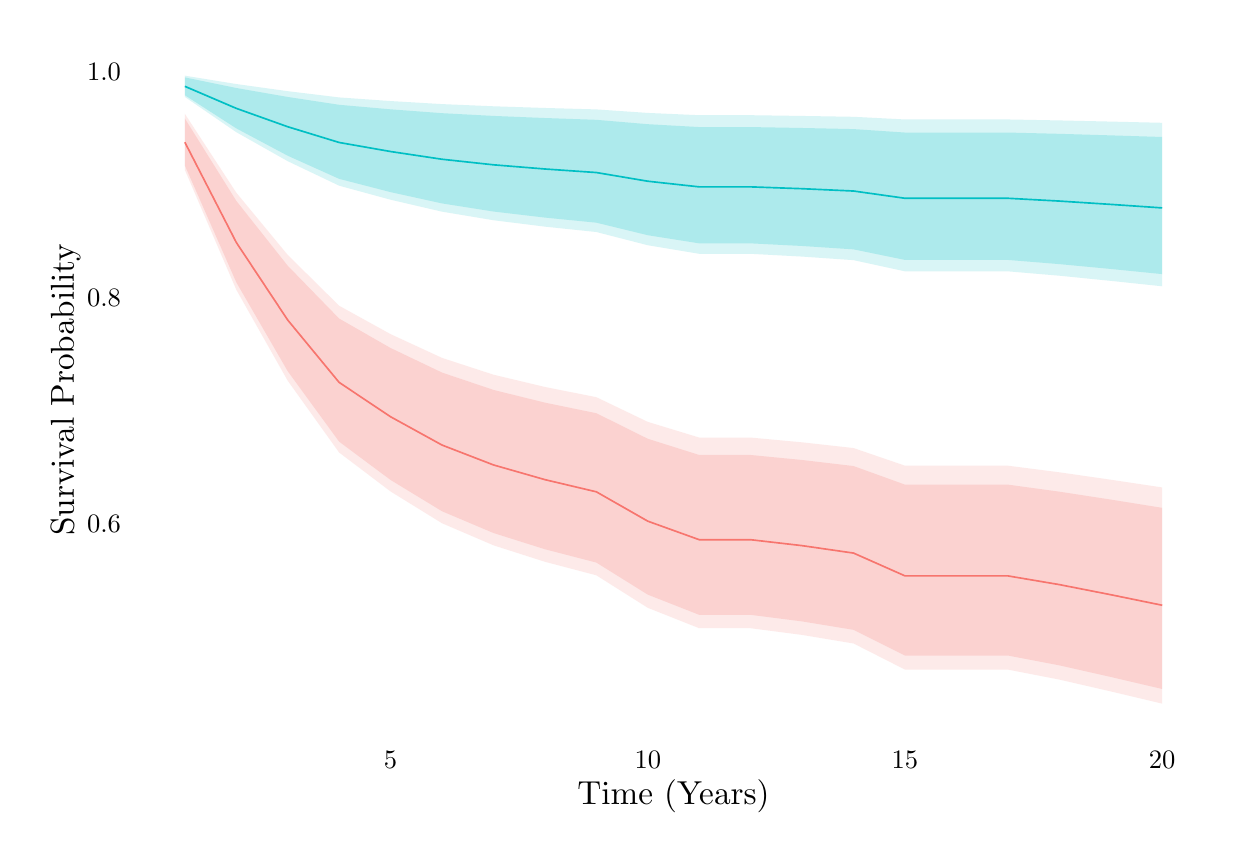
\begin{tikzpicture}[x=1pt,y=1pt]
\definecolor[named]{drawColor}{rgb}{0.00,0.00,0.00}
\definecolor[named]{fillColor}{rgb}{1.00,1.00,1.00}
\fill[color=fillColor,] (0,0) rectangle (433.62,289.08);
\begin{scope}
\path[clip] (  0.00,  0.00) rectangle (433.62,289.08);
\end{scope}
\begin{scope}
\path[clip] (  0.00,  0.00) rectangle (433.62,289.08);
\end{scope}
\begin{scope}
\path[clip] (  0.00,  0.00) rectangle (433.62,289.08);
\end{scope}
\begin{scope}
\path[clip] (  0.00,  0.00) rectangle (433.62,289.08);
\end{scope}
\begin{scope}
\path[clip] (  0.00,  0.00) rectangle (433.62,289.08);
\end{scope}
\begin{scope}
\path[clip] (  0.00,  0.00) rectangle (433.62,289.08);
\end{scope}
\begin{scope}
\path[clip] (  0.00,  0.00) rectangle (433.62,289.08);
\end{scope}
\begin{scope}
\path[clip] (  0.00,  0.00) rectangle (433.62,289.08);
\end{scope}
\begin{scope}
\path[clip] (  0.00,  0.00) rectangle (433.62,289.08);
\end{scope}
\begin{scope}
\path[clip] (  0.00,  0.00) rectangle (433.62,289.08);
\definecolor[named]{drawColor}{rgb}{1.00,1.00,1.00}
\definecolor[named]{fillColor}{rgb}{1.00,1.00,1.00}

\draw[color=drawColor,line width= 0.6pt,line cap=round,line join=round,fill=fillColor,] (  0.00,  0.00) rectangle (433.62,289.08);
\end{scope}
\begin{scope}
\path[clip] (  0.00,  0.00) rectangle (433.62,289.08);
\end{scope}
\begin{scope}
\path[clip] (  0.00,  0.00) rectangle (433.62,289.08);
\end{scope}
\begin{scope}
\path[clip] (  0.00,  0.00) rectangle (433.62,289.08);
\end{scope}
\begin{scope}
\path[clip] ( 39.13, 33.48) rectangle (427.62,283.08);
\definecolor[named]{fillColor}{rgb}{1.00,1.00,1.00}

\draw[fill=fillColor,draw opacity=0.00,] ( 39.13, 33.48) rectangle (427.62,283.08);
\definecolor[named]{drawColor}{rgb}{0.97,0.46,0.43}
\definecolor[named]{fillColor}{rgb}{0.97,0.46,0.43}

\draw[color=drawColor,line width= 0.6pt,line join=round,] ( 56.79,247.68) --
	( 75.38,211.48) --
	( 93.96,183.44) --
	(112.55,160.89) --
	(131.14,148.48) --
	(149.73,138.25) --
	(168.32,131.07) --
	(186.90,125.76) --
	(205.49,121.36) --
	(224.08,110.75) --
	(242.67,104.05) --
	(261.26,104.05) --
	(279.84,101.91) --
	(298.43, 99.22) --
	(317.02, 90.98) --
	(335.61, 90.98) --
	(354.20, 90.98) --
	(372.79, 87.83) --
	(391.37, 84.18) --
	(409.96, 80.37);
\definecolor[named]{drawColor}{rgb}{0.00,0.75,0.77}
\definecolor[named]{fillColor}{rgb}{0.00,0.75,0.77}

\draw[color=drawColor,line width= 0.6pt,line join=round,] ( 56.79,267.88) --
	( 75.38,259.92) --
	( 93.96,253.28) --
	(112.55,247.59) --
	(131.14,244.32) --
	(149.73,241.53) --
	(168.32,239.52) --
	(186.90,238.01) --
	(205.49,236.73) --
	(224.08,233.59) --
	(242.67,231.55) --
	(261.26,231.55) --
	(279.84,230.89) --
	(298.43,230.05) --
	(317.02,227.43) --
	(335.61,227.43) --
	(354.20,227.43) --
	(372.79,226.42) --
	(391.37,225.22) --
	(409.96,223.95);
\definecolor[named]{fillColor}{rgb}{0.97,0.46,0.43}

\draw[fill=fillColor,fill opacity=0.15,draw opacity=0.00,] ( 56.79,257.94) --
	( 75.38,229.45) --
	( 93.96,206.96) --
	(112.55,188.59) --
	(131.14,178.33) --
	(149.73,169.75) --
	(168.32,163.68) --
	(186.90,159.25) --
	(205.49,155.55) --
	(224.08,146.63) --
	(242.67,140.96) --
	(261.26,140.96) --
	(279.84,139.24) --
	(298.43,137.17) --
	(317.02,130.80) --
	(335.61,130.80) --
	(354.20,130.80) --
	(372.79,128.41) --
	(391.37,125.73) --
	(409.96,122.94) --
	(409.96, 44.82) --
	(391.37, 49.24) --
	(372.79, 53.51) --
	(354.20, 57.12) --
	(335.61, 57.12) --
	(317.02, 57.12) --
	(298.43, 66.56) --
	(279.84, 69.65) --
	(261.26, 72.07) --
	(242.67, 72.07) --
	(224.08, 79.44) --
	(205.49, 91.19) --
	(186.90, 96.08) --
	(168.32,102.03) --
	(149.73,110.00) --
	(131.14,121.48) --
	(112.55,135.56) --
	( 93.96,161.53) --
	( 75.38,194.40) --
	( 56.79,237.69) --
	cycle;
\definecolor[named]{fillColor}{rgb}{0.00,0.75,0.77}

\draw[fill=fillColor,fill opacity=0.15,draw opacity=0.00,] ( 56.79,271.73) --
	( 75.38,268.71) --
	( 93.96,266.13) --
	(112.55,263.87) --
	(131.14,262.56) --
	(149.73,261.46) --
	(168.32,260.67) --
	(186.90,260.06) --
	(205.49,259.54) --
	(224.08,258.27) --
	(242.67,257.45) --
	(261.26,257.45) --
	(279.84,257.18) --
	(298.43,256.87) --
	(317.02,255.91) --
	(335.61,255.91) --
	(354.20,255.91) --
	(372.79,255.56) --
	(391.37,255.14) --
	(409.96,254.70) --
	(409.96,195.63) --
	(391.37,197.59) --
	(372.79,199.45) --
	(354.20,201.03) --
	(335.61,201.03) --
	(317.02,201.03) --
	(298.43,205.07) --
	(279.84,206.36) --
	(261.26,207.36) --
	(242.67,207.36) --
	(224.08,210.46) --
	(205.49,215.24) --
	(186.90,217.18) --
	(168.32,219.50) --
	(149.73,222.59) --
	(131.14,226.91) --
	(112.55,231.98) --
	( 93.96,240.84) --
	( 75.38,251.32) --
	( 56.79,264.06) --
	cycle;
\definecolor[named]{fillColor}{rgb}{0.97,0.46,0.43}

\draw[fill=fillColor,fill opacity=0.20,draw opacity=0.00,] ( 56.79,256.27) --
	( 75.38,226.50) --
	( 93.96,203.06) --
	(112.55,183.96) --
	(131.14,173.33) --
	(149.73,164.45) --
	(168.32,158.18) --
	(186.90,153.59) --
	(205.49,149.76) --
	(224.08,140.53) --
	(242.67,134.67) --
	(261.26,134.67) --
	(279.84,132.86) --
	(298.43,130.67) --
	(317.02,123.96) --
	(335.61,123.96) --
	(354.20,123.96) --
	(372.79,121.42) --
	(391.37,118.56) --
	(409.96,115.57) --
	(409.96, 50.11) --
	(391.37, 54.46) --
	(372.79, 58.65) --
	(354.20, 62.20) --
	(335.61, 62.20) --
	(317.02, 62.20) --
	(298.43, 71.48) --
	(279.84, 74.53) --
	(261.26, 76.90) --
	(242.67, 76.90) --
	(224.08, 84.20) --
	(205.49, 95.79) --
	(186.90,100.61) --
	(168.32,106.47) --
	(149.73,114.33) --
	(131.14,125.64) --
	(112.55,139.48) --
	( 93.96,164.95) --
	( 75.38,197.08) --
	( 56.79,239.28) --
	cycle;
\definecolor[named]{fillColor}{rgb}{0.00,0.75,0.77}

\draw[fill=fillColor,fill opacity=0.20,draw opacity=0.00,] ( 56.79,271.11) --
	( 75.38,267.28) --
	( 93.96,264.04) --
	(112.55,261.21) --
	(131.14,259.57) --
	(149.73,258.18) --
	(168.32,257.19) --
	(186.90,256.43) --
	(205.49,255.78) --
	(224.08,254.20) --
	(242.67,253.16) --
	(261.26,253.16) --
	(279.84,252.83) --
	(298.43,252.43) --
	(317.02,251.18) --
	(335.61,251.18) --
	(354.20,251.18) --
	(372.79,250.72) --
	(391.37,250.16) --
	(409.96,249.58) --
	(409.96,200.03) --
	(391.37,201.89) --
	(372.79,203.64) --
	(354.20,205.15) --
	(335.61,205.15) --
	(317.02,205.15) --
	(298.43,208.97) --
	(279.84,210.19) --
	(261.26,211.14) --
	(242.67,211.14) --
	(224.08,214.08) --
	(205.49,218.61) --
	(186.90,220.45) --
	(168.32,222.64) --
	(149.73,225.57) --
	(131.14,229.65) --
	(112.55,234.45) --
	( 93.96,242.81) --
	( 75.38,252.69) --
	( 56.79,264.67) --
	cycle;
\end{scope}
\begin{scope}
\path[clip] (  0.00,  0.00) rectangle (433.62,289.08);
\end{scope}
\begin{scope}
\path[clip] (  0.00,  0.00) rectangle (433.62,289.08);
\end{scope}
\begin{scope}
\path[clip] (  0.00,  0.00) rectangle (433.62,289.08);
\end{scope}
\begin{scope}
\path[clip] (  0.00,  0.00) rectangle (433.62,289.08);
\end{scope}
\begin{scope}
\path[clip] (  0.00,  0.00) rectangle (433.62,289.08);
\end{scope}
\begin{scope}
\path[clip] (  0.00,  0.00) rectangle (433.62,289.08);
\definecolor[named]{drawColor}{rgb}{0.00,0.00,0.00}

\node[color=drawColor,anchor=base east,inner sep=0pt, outer sep=0pt, scale=  0.96] at ( 33.73,106.51) {0.6%
};

\node[color=drawColor,anchor=base east,inner sep=0pt, outer sep=0pt, scale=  0.96] at ( 33.73,188.16) {0.8%
};

\node[color=drawColor,anchor=base east,inner sep=0pt, outer sep=0pt, scale=  0.96] at ( 33.73,269.81) {1.0%
};
\end{scope}
\begin{scope}
\path[clip] (  0.00,  0.00) rectangle (433.62,289.08);
\end{scope}
\begin{scope}
\path[clip] (  0.00,  0.00) rectangle (433.62,289.08);
\end{scope}
\begin{scope}
\path[clip] (  0.00,  0.00) rectangle (433.62,289.08);
\end{scope}
\begin{scope}
\path[clip] (  0.00,  0.00) rectangle (433.62,289.08);
\end{scope}
\begin{scope}
\path[clip] (  0.00,  0.00) rectangle (433.62,289.08);
\end{scope}
\begin{scope}
\path[clip] (  0.00,  0.00) rectangle (433.62,289.08);
\end{scope}
\begin{scope}
\path[clip] (  0.00,  0.00) rectangle (433.62,289.08);
\end{scope}
\begin{scope}
\path[clip] (  0.00,  0.00) rectangle (433.62,289.08);
\end{scope}
\begin{scope}
\path[clip] (  0.00,  0.00) rectangle (433.62,289.08);
\end{scope}
\begin{scope}
\path[clip] (  0.00,  0.00) rectangle (433.62,289.08);
\end{scope}
\begin{scope}
\path[clip] (  0.00,  0.00) rectangle (433.62,289.08);
\end{scope}
\begin{scope}
\path[clip] (  0.00,  0.00) rectangle (433.62,289.08);
\definecolor[named]{drawColor}{rgb}{0.00,0.00,0.00}

\node[color=drawColor,anchor=base,inner sep=0pt, outer sep=0pt, scale=  0.96] at (131.14, 21.46) {5%
};

\node[color=drawColor,anchor=base,inner sep=0pt, outer sep=0pt, scale=  0.96] at (224.08, 21.46) {10%
};

\node[color=drawColor,anchor=base,inner sep=0pt, outer sep=0pt, scale=  0.96] at (317.02, 21.46) {15%
};

\node[color=drawColor,anchor=base,inner sep=0pt, outer sep=0pt, scale=  0.96] at (409.96, 21.46) {20%
};
\end{scope}
\begin{scope}
\path[clip] (  0.00,  0.00) rectangle (433.62,289.08);
\end{scope}
\begin{scope}
\path[clip] (  0.00,  0.00) rectangle (433.62,289.08);
\end{scope}
\begin{scope}
\path[clip] (  0.00,  0.00) rectangle (433.62,289.08);
\end{scope}
\begin{scope}
\path[clip] (  0.00,  0.00) rectangle (433.62,289.08);
\definecolor[named]{drawColor}{rgb}{0.00,0.00,0.00}

\node[color=drawColor,anchor=base,inner sep=0pt, outer sep=0pt, scale=  1.20] at (233.37,  8.40) {Time (Years)%
};
\end{scope}
\begin{scope}
\path[clip] (  0.00,  0.00) rectangle (433.62,289.08);
\end{scope}
\begin{scope}
\path[clip] (  0.00,  0.00) rectangle (433.62,289.08);
\definecolor[named]{drawColor}{rgb}{0.00,0.00,0.00}

\node[rotate= 90.00,color=drawColor,anchor=base,inner sep=0pt, outer sep=0pt, scale=  1.20] at ( 16.66,158.28) {Survival Probability%
};
\end{scope}
\begin{scope}
\path[clip] (  0.00,  0.00) rectangle (433.62,289.08);
\end{scope}
\begin{scope}
\path[clip] (  0.00,  0.00) rectangle (433.62,289.08);
\end{scope}
\begin{scope}
\path[clip] (  0.00,  0.00) rectangle (433.62,289.08);
\end{scope}
\begin{scope}
\path[clip] (  0.00,  0.00) rectangle (433.62,289.08);
\end{scope}
\end{tikzpicture}
}
		\label{fig:compSancSurv}}	

	\end{tabular}

	\label{fig:surv3}	
\end{figure}


Our sanction reciprocity measure tells a similar story, but focuses on the consequences of past reciprocal adverse relations. Here we can see that countries whom have sanctioned each other in the past without complying to one another are not likely to comply with one another in the present. On the right side of Figure~\ref{fig:surv3}, we can again demonstrate that within just five years the probability of non-compliance in a case where target and sender states have not had adverse past relations is half compared to a case where past adverse relations are present. This points to important consequences for sender states, namely that the continuous sanctioning of a particular state without previous compliance from the target state may build up the target's resistance to comply with future sanctions.

\subsection*{Performance}

To assess the accuracy and performance of these estimates we employ a six-fold cross validation procedure.\footnote{Results of analysis were similar when employing a 10-fold cross validation as well, however, we limit to showing six here due to space limitations.} We use this procedure both to determine the robustness of our coefficient estimates when estimated on different subsamples of our dataset, and to assess how well the results of our model would generalize to an independent dataset. To begin the cross-validation, we split the sanction cases in our dataset into six approximately equal subsets. We then run each model shown in Table~\ref{tab:regResults} six times, where in each iteration we left out one subsample to use as a test set. This allows us to compare the prediction accuracy of each model, thereby helping us to determine the gains from incorporating the reciprocity covariates that are key to our argument.

First, however, we show the results for our reciprocity covariates when we rerun our survival analysis on each of the six folds from the cross-validation. This analysis helps us to understand whether some of the subsets in our dataset follow a different pattern than what is in the broader set.\footnote{See \cite{beck2008time} for more on this approach.} Figure~\ref{fig:crossval} shows that this is not the case for the analysis we present here, the coefficient estimates for compliance and sanction reciprocity remain consistent across each of these subsamples.\footnote{The parameter estimates for the other covariates also remain consistent across each of the six folds but we leave them out here due to space constraints.}


\begin{figure}[ht]
	\centering
	\caption{Reciprocity coefficient estimates from each of the six-folds of the cross validation procedure.}
	\resizebox{1\textwidth}{!}{% Created by tikzDevice version 0.7.0 on 2014-08-02 16:07:02
% !TEX encoding = UTF-8 Unicode
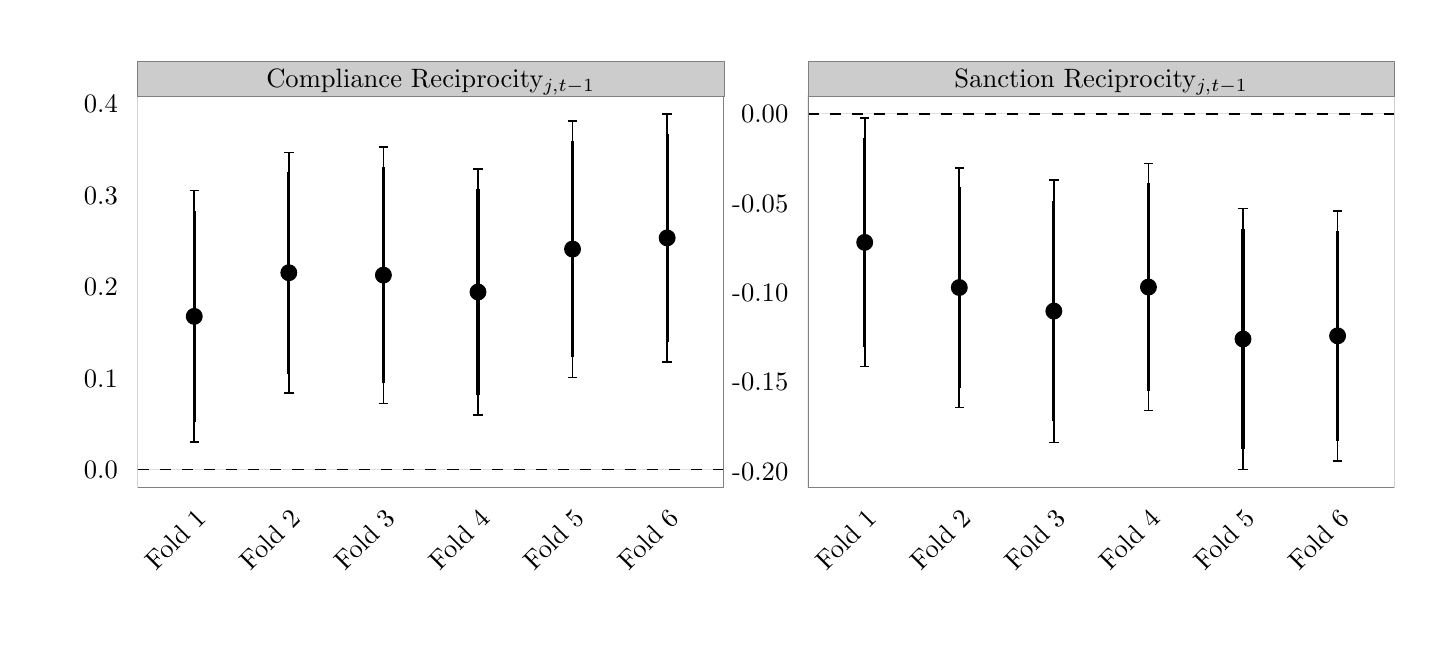
\begin{tikzpicture}[x=1pt,y=1pt]
\definecolor[named]{fillColor}{rgb}{1.00,1.00,1.00}
\path[use as bounding box,fill=fillColor,fill opacity=0.00] (0,0) rectangle (505.89,216.81);
\begin{scope}
\path[clip] (  0.00,  0.00) rectangle (505.89,216.81);
\definecolor[named]{drawColor}{rgb}{1.00,1.00,1.00}
\definecolor[named]{fillColor}{rgb}{1.00,1.00,1.00}

\path[draw=drawColor,line width= 0.6pt,line join=round,line cap=round,fill=fillColor] (  0.00,  0.00) rectangle (505.89,216.81);
\end{scope}
\begin{scope}
\path[clip] ( 39.69, 50.67) rectangle (251.57,192.13);
\definecolor[named]{fillColor}{rgb}{1.00,1.00,1.00}

\path[fill=fillColor] ( 39.69, 50.67) rectangle (251.57,192.13);
\definecolor[named]{drawColor}{rgb}{0.00,0.00,0.00}
\definecolor[named]{fillColor}{rgb}{0.00,0.00,0.00}

\path[draw=drawColor,draw opacity=0.30,line width= 0.3pt,line join=round,fill=fillColor,fill opacity=0.30] ( 60.19, 67.01) -- ( 60.19,157.97);

\path[draw=drawColor,draw opacity=0.30,line width= 0.3pt,line join=round,fill=fillColor,fill opacity=0.30] ( 94.37, 84.84) -- ( 94.37,171.68);

\path[draw=drawColor,draw opacity=0.30,line width= 0.3pt,line join=round,fill=fillColor,fill opacity=0.30] (128.54, 81.00) -- (128.54,173.77);

\path[draw=drawColor,draw opacity=0.30,line width= 0.3pt,line join=round,fill=fillColor,fill opacity=0.30] (162.72, 76.75) -- (162.72,165.85);

\path[draw=drawColor,draw opacity=0.30,line width= 0.3pt,line join=round,fill=fillColor,fill opacity=0.30] (196.89, 90.43) -- (196.89,183.18);

\path[draw=drawColor,draw opacity=0.30,line width= 0.3pt,line join=round,fill=fillColor,fill opacity=0.30] (231.07, 95.99) -- (231.07,185.70);
\definecolor[named]{drawColor}{rgb}{0.00,0.00,0.00}
\definecolor[named]{fillColor}{rgb}{0.00,0.00,0.00}

\path[draw=drawColor,line width= 1.1pt,line join=round,fill=fillColor] ( 60.19, 74.32) -- ( 60.19,150.66);

\path[draw=drawColor,line width= 1.1pt,line join=round,fill=fillColor] ( 94.37, 91.82) -- ( 94.37,164.70);

\path[draw=drawColor,line width= 1.1pt,line join=round,fill=fillColor] (128.54, 88.46) -- (128.54,166.31);

\path[draw=drawColor,line width= 1.1pt,line join=round,fill=fillColor] (162.72, 83.91) -- (162.72,158.69);

\path[draw=drawColor,line width= 1.1pt,line join=round,fill=fillColor] (196.89, 97.88) -- (196.89,175.73);

\path[draw=drawColor,line width= 1.1pt,line join=round,fill=fillColor] (231.07,103.20) -- (231.07,178.49);

\path[draw=drawColor,line width= 0.6pt,dash pattern=on 4pt off 4pt ,line join=round,fill=fillColor] ( 39.69, 57.10) -- (251.57, 57.10);

\path[draw=drawColor,line width= 0.4pt,line join=round,line cap=round,fill=fillColor] ( 60.19,112.49) circle (  2.85);

\path[draw=drawColor,line width= 0.4pt,line join=round,line cap=round,fill=fillColor] ( 94.37,128.26) circle (  2.85);

\path[draw=drawColor,line width= 0.4pt,line join=round,line cap=round,fill=fillColor] (128.54,127.39) circle (  2.85);

\path[draw=drawColor,line width= 0.4pt,line join=round,line cap=round,fill=fillColor] (162.72,121.30) circle (  2.85);

\path[draw=drawColor,line width= 0.4pt,line join=round,line cap=round,fill=fillColor] (196.89,136.80) circle (  2.85);

\path[draw=drawColor,line width= 0.4pt,line join=round,line cap=round,fill=fillColor] (231.07,140.84) circle (  2.85);

\path[draw=drawColor,line width= 0.6pt,line join=round] ( 58.48,157.97) --
	( 61.90,157.97);

\path[draw=drawColor,line width= 0.6pt,line join=round] ( 60.19,157.97) --
	( 60.19, 67.01);

\path[draw=drawColor,line width= 0.6pt,line join=round] ( 58.48, 67.01) --
	( 61.90, 67.01);

\path[draw=drawColor,line width= 0.6pt,line join=round] ( 92.66,171.68) --
	( 96.08,171.68);

\path[draw=drawColor,line width= 0.6pt,line join=round] ( 94.37,171.68) --
	( 94.37, 84.84);

\path[draw=drawColor,line width= 0.6pt,line join=round] ( 92.66, 84.84) --
	( 96.08, 84.84);

\path[draw=drawColor,line width= 0.6pt,line join=round] (126.83,173.77) --
	(130.25,173.77);

\path[draw=drawColor,line width= 0.6pt,line join=round] (128.54,173.77) --
	(128.54, 81.00);

\path[draw=drawColor,line width= 0.6pt,line join=round] (126.83, 81.00) --
	(130.25, 81.00);

\path[draw=drawColor,line width= 0.6pt,line join=round] (161.01,165.85) --
	(164.43,165.85);

\path[draw=drawColor,line width= 0.6pt,line join=round] (162.72,165.85) --
	(162.72, 76.75);

\path[draw=drawColor,line width= 0.6pt,line join=round] (161.01, 76.75) --
	(164.43, 76.75);

\path[draw=drawColor,line width= 0.6pt,line join=round] (195.18,183.18) --
	(198.60,183.18);

\path[draw=drawColor,line width= 0.6pt,line join=round] (196.89,183.18) --
	(196.89, 90.43);

\path[draw=drawColor,line width= 0.6pt,line join=round] (195.18, 90.43) --
	(198.60, 90.43);

\path[draw=drawColor,line width= 0.6pt,line join=round] (229.36,185.70) --
	(232.78,185.70);

\path[draw=drawColor,line width= 0.6pt,line join=round] (231.07,185.70) --
	(231.07, 95.99);

\path[draw=drawColor,line width= 0.6pt,line join=round] (229.36, 95.99) --
	(232.78, 95.99);
\definecolor[named]{drawColor}{rgb}{0.50,0.50,0.50}

\path[draw=drawColor,line width= 0.6pt,line join=round,line cap=round] ( 39.69, 50.67) rectangle (251.57,192.13);
\end{scope}
\begin{scope}
\path[clip] (281.96, 50.67) rectangle (493.85,192.13);
\definecolor[named]{fillColor}{rgb}{1.00,1.00,1.00}

\path[fill=fillColor] (281.96, 50.67) rectangle (493.85,192.13);
\definecolor[named]{drawColor}{rgb}{0.00,0.00,0.00}
\definecolor[named]{fillColor}{rgb}{0.00,0.00,0.00}

\path[draw=drawColor,draw opacity=0.30,line width= 0.3pt,line join=round,fill=fillColor,fill opacity=0.30] (302.46, 94.34) -- (302.46,184.13);

\path[draw=drawColor,draw opacity=0.30,line width= 0.3pt,line join=round,fill=fillColor,fill opacity=0.30] (336.64, 79.61) -- (336.64,166.21);

\path[draw=drawColor,draw opacity=0.30,line width= 0.3pt,line join=round,fill=fillColor,fill opacity=0.30] (370.81, 66.95) -- (370.81,161.82);

\path[draw=drawColor,draw opacity=0.30,line width= 0.3pt,line join=round,fill=fillColor,fill opacity=0.30] (404.99, 78.48) -- (404.99,167.69);

\path[draw=drawColor,draw opacity=0.30,line width= 0.3pt,line join=round,fill=fillColor,fill opacity=0.30] (439.16, 57.10) -- (439.16,151.50);

\path[draw=drawColor,draw opacity=0.30,line width= 0.3pt,line join=round,fill=fillColor,fill opacity=0.30] (473.34, 60.25) -- (473.34,150.65);
\definecolor[named]{drawColor}{rgb}{0.00,0.00,0.00}
\definecolor[named]{fillColor}{rgb}{0.00,0.00,0.00}

\path[draw=drawColor,line width= 1.1pt,line join=round,fill=fillColor] (302.46,101.55) -- (302.46,176.91);

\path[draw=drawColor,line width= 1.1pt,line join=round,fill=fillColor] (336.64, 86.57) -- (336.64,159.25);

\path[draw=drawColor,line width= 1.1pt,line join=round,fill=fillColor] (370.81, 74.58) -- (370.81,154.20);

\path[draw=drawColor,line width= 1.1pt,line join=round,fill=fillColor] (404.99, 85.65) -- (404.99,160.52);

\path[draw=drawColor,line width= 1.1pt,line join=round,fill=fillColor] (439.16, 64.69) -- (439.16,143.91);

\path[draw=drawColor,line width= 1.1pt,line join=round,fill=fillColor] (473.34, 67.52) -- (473.34,143.38);

\path[draw=drawColor,line width= 0.6pt,dash pattern=on 4pt off 4pt ,line join=round,fill=fillColor] (281.96,185.70) -- (493.85,185.70);

\path[draw=drawColor,line width= 0.4pt,line join=round,line cap=round,fill=fillColor] (302.46,139.23) circle (  2.85);

\path[draw=drawColor,line width= 0.4pt,line join=round,line cap=round,fill=fillColor] (336.64,122.91) circle (  2.85);

\path[draw=drawColor,line width= 0.4pt,line join=round,line cap=round,fill=fillColor] (370.81,114.39) circle (  2.85);

\path[draw=drawColor,line width= 0.4pt,line join=round,line cap=round,fill=fillColor] (404.99,123.08) circle (  2.85);

\path[draw=drawColor,line width= 0.4pt,line join=round,line cap=round,fill=fillColor] (439.16,104.30) circle (  2.85);

\path[draw=drawColor,line width= 0.4pt,line join=round,line cap=round,fill=fillColor] (473.34,105.45) circle (  2.85);

\path[draw=drawColor,line width= 0.6pt,line join=round] (300.76,184.13) --
	(304.17,184.13);

\path[draw=drawColor,line width= 0.6pt,line join=round] (302.46,184.13) --
	(302.46, 94.34);

\path[draw=drawColor,line width= 0.6pt,line join=round] (300.76, 94.34) --
	(304.17, 94.34);

\path[draw=drawColor,line width= 0.6pt,line join=round] (334.93,166.21) --
	(338.35,166.21);

\path[draw=drawColor,line width= 0.6pt,line join=round] (336.64,166.21) --
	(336.64, 79.61);

\path[draw=drawColor,line width= 0.6pt,line join=round] (334.93, 79.61) --
	(338.35, 79.61);

\path[draw=drawColor,line width= 0.6pt,line join=round] (369.11,161.82) --
	(372.52,161.82);

\path[draw=drawColor,line width= 0.6pt,line join=round] (370.81,161.82) --
	(370.81, 66.95);

\path[draw=drawColor,line width= 0.6pt,line join=round] (369.11, 66.95) --
	(372.52, 66.95);

\path[draw=drawColor,line width= 0.6pt,line join=round] (403.28,167.69) --
	(406.70,167.69);

\path[draw=drawColor,line width= 0.6pt,line join=round] (404.99,167.69) --
	(404.99, 78.48);

\path[draw=drawColor,line width= 0.6pt,line join=round] (403.28, 78.48) --
	(406.70, 78.48);

\path[draw=drawColor,line width= 0.6pt,line join=round] (437.46,151.50) --
	(440.87,151.50);

\path[draw=drawColor,line width= 0.6pt,line join=round] (439.16,151.50) --
	(439.16, 57.10);

\path[draw=drawColor,line width= 0.6pt,line join=round] (437.46, 57.10) --
	(440.87, 57.10);

\path[draw=drawColor,line width= 0.6pt,line join=round] (471.63,150.65) --
	(475.05,150.65);

\path[draw=drawColor,line width= 0.6pt,line join=round] (473.34,150.65) --
	(473.34, 60.25);

\path[draw=drawColor,line width= 0.6pt,line join=round] (471.63, 60.25) --
	(475.05, 60.25);
\definecolor[named]{drawColor}{rgb}{0.50,0.50,0.50}

\path[draw=drawColor,line width= 0.6pt,line join=round,line cap=round] (281.96, 50.67) rectangle (493.85,192.13);
\end{scope}
\begin{scope}
\path[clip] (  0.00,  0.00) rectangle (505.89,216.81);
\definecolor[named]{drawColor}{rgb}{0.50,0.50,0.50}
\definecolor[named]{fillColor}{rgb}{0.80,0.80,0.80}

\path[draw=drawColor,line width= 0.2pt,line join=round,line cap=round,fill=fillColor] ( 39.69,192.13) rectangle (251.57,204.77);
\definecolor[named]{drawColor}{rgb}{0.00,0.00,0.00}

\node[text=drawColor,anchor=base,inner sep=0pt, outer sep=0pt, scale=  0.96] at (145.63,195.14) {Compliance Reciprocity$_{j,t-1}$};
\end{scope}
\begin{scope}
\path[clip] (  0.00,  0.00) rectangle (505.89,216.81);
\definecolor[named]{drawColor}{rgb}{0.50,0.50,0.50}
\definecolor[named]{fillColor}{rgb}{0.80,0.80,0.80}

\path[draw=drawColor,line width= 0.2pt,line join=round,line cap=round,fill=fillColor] (281.96,192.13) rectangle (493.85,204.77);
\definecolor[named]{drawColor}{rgb}{0.00,0.00,0.00}

\node[text=drawColor,anchor=base,inner sep=0pt, outer sep=0pt, scale=  0.96] at (387.90,195.14) {Sanction Reciprocity$_{j,t-1}$};
\end{scope}
\begin{scope}
\path[clip] (  0.00,  0.00) rectangle (505.89,216.81);
\definecolor[named]{drawColor}{rgb}{0.00,0.00,0.00}

\node[text=drawColor,anchor=base east,inner sep=0pt, outer sep=0pt, scale=  0.96] at ( 32.57, 53.79) {0.0};

\node[text=drawColor,anchor=base east,inner sep=0pt, outer sep=0pt, scale=  0.96] at ( 32.57, 86.88) {0.1};

\node[text=drawColor,anchor=base east,inner sep=0pt, outer sep=0pt, scale=  0.96] at ( 32.57,119.97) {0.2};

\node[text=drawColor,anchor=base east,inner sep=0pt, outer sep=0pt, scale=  0.96] at ( 32.57,153.05) {0.3};

\node[text=drawColor,anchor=base east,inner sep=0pt, outer sep=0pt, scale=  0.96] at ( 32.57,186.14) {0.4};
\end{scope}
\begin{scope}
\path[clip] (  0.00,  0.00) rectangle (505.89,216.81);
\definecolor[named]{drawColor}{rgb}{0.00,0.00,0.00}

\node[text=drawColor,anchor=base east,inner sep=0pt, outer sep=0pt, scale=  0.96] at (274.85, 53.29) {-0.20};

\node[text=drawColor,anchor=base east,inner sep=0pt, outer sep=0pt, scale=  0.96] at (274.85, 85.57) {-0.15};

\node[text=drawColor,anchor=base east,inner sep=0pt, outer sep=0pt, scale=  0.96] at (274.85,117.84) {-0.10};

\node[text=drawColor,anchor=base east,inner sep=0pt, outer sep=0pt, scale=  0.96] at (274.85,150.12) {-0.05};

\node[text=drawColor,anchor=base east,inner sep=0pt, outer sep=0pt, scale=  0.96] at (274.85,182.39) {0.00};
\end{scope}
\begin{scope}
\path[clip] (  0.00,  0.00) rectangle (505.89,216.81);
\definecolor[named]{drawColor}{rgb}{0.00,0.00,0.00}

\node[text=drawColor,rotate= 45.00,anchor=base east,inner sep=0pt, outer sep=0pt, scale=  0.96] at ( 64.87, 38.88) {Fold 1};

\node[text=drawColor,rotate= 45.00,anchor=base east,inner sep=0pt, outer sep=0pt, scale=  0.96] at ( 99.04, 38.88) {Fold 2};

\node[text=drawColor,rotate= 45.00,anchor=base east,inner sep=0pt, outer sep=0pt, scale=  0.96] at (133.22, 38.88) {Fold 3};

\node[text=drawColor,rotate= 45.00,anchor=base east,inner sep=0pt, outer sep=0pt, scale=  0.96] at (167.39, 38.88) {Fold 4};

\node[text=drawColor,rotate= 45.00,anchor=base east,inner sep=0pt, outer sep=0pt, scale=  0.96] at (201.57, 38.88) {Fold 5};

\node[text=drawColor,rotate= 45.00,anchor=base east,inner sep=0pt, outer sep=0pt, scale=  0.96] at (235.74, 38.88) {Fold 6};
\end{scope}
\begin{scope}
\path[clip] (  0.00,  0.00) rectangle (505.89,216.81);
\definecolor[named]{drawColor}{rgb}{0.00,0.00,0.00}

\node[text=drawColor,rotate= 45.00,anchor=base east,inner sep=0pt, outer sep=0pt, scale=  0.96] at (307.14, 38.88) {Fold 1};

\node[text=drawColor,rotate= 45.00,anchor=base east,inner sep=0pt, outer sep=0pt, scale=  0.96] at (341.31, 38.88) {Fold 2};

\node[text=drawColor,rotate= 45.00,anchor=base east,inner sep=0pt, outer sep=0pt, scale=  0.96] at (375.49, 38.88) {Fold 3};

\node[text=drawColor,rotate= 45.00,anchor=base east,inner sep=0pt, outer sep=0pt, scale=  0.96] at (409.66, 38.88) {Fold 4};

\node[text=drawColor,rotate= 45.00,anchor=base east,inner sep=0pt, outer sep=0pt, scale=  0.96] at (443.84, 38.88) {Fold 5};

\node[text=drawColor,rotate= 45.00,anchor=base east,inner sep=0pt, outer sep=0pt, scale=  0.96] at (478.02, 38.88) {Fold 6};
\end{scope}
\end{tikzpicture}
}
	\label{fig:crossval}
\end{figure}


A key question that remains, however, is whether we are able to better explain sanction compliance through the incorporation of these network level covariates. Figure~\ref{fig:auc} shows out-of-sample time-dependent AUC (Area Under the Curve) results from the six-fold cross validation procedure. When calculating the time-dependent AUC we vary the time parameter to range from 0 to 15 years.\footnote{Time-dependent AUCs were computed using the formula provided by \citet{chambless2006estimation}.} We set the max for 15 years because only 4\% of sanction cases in our dataset that extend past 15 years end with compliance by a target state. This leads to the AUC statistics for each model. After that time point, the accuracy of any of the models begin to coalesce. Before the 15 year mark, however, we see considerable variation in the time-dependent AUC statistics for each model. Most importantly, we can see that Model 3, where we incorporate our network level covariates, provides a noticeably higher AUC than the alternatives that we examined. Even simply accounting for proximate relationships, as we did in Model 2, does not provide a noticeably higher level of performance than target-state focused explanations.

\begin{figure}[ht]
	\centering
	\caption{Out-of-sample time-dependent AUC statistics from six-fold cross validation procedure for each model shown in Table~\ref{tab:regResults}. The solid line represents Model 1, the dotted line represents Model 2, and the dashed line represents Model 3.}
	\resizebox{1\textwidth}{!}{% Created by tikzDevice version 0.6.1 on 2016-06-13 09:53:06
% !TEX encoding = UTF-8 Unicode
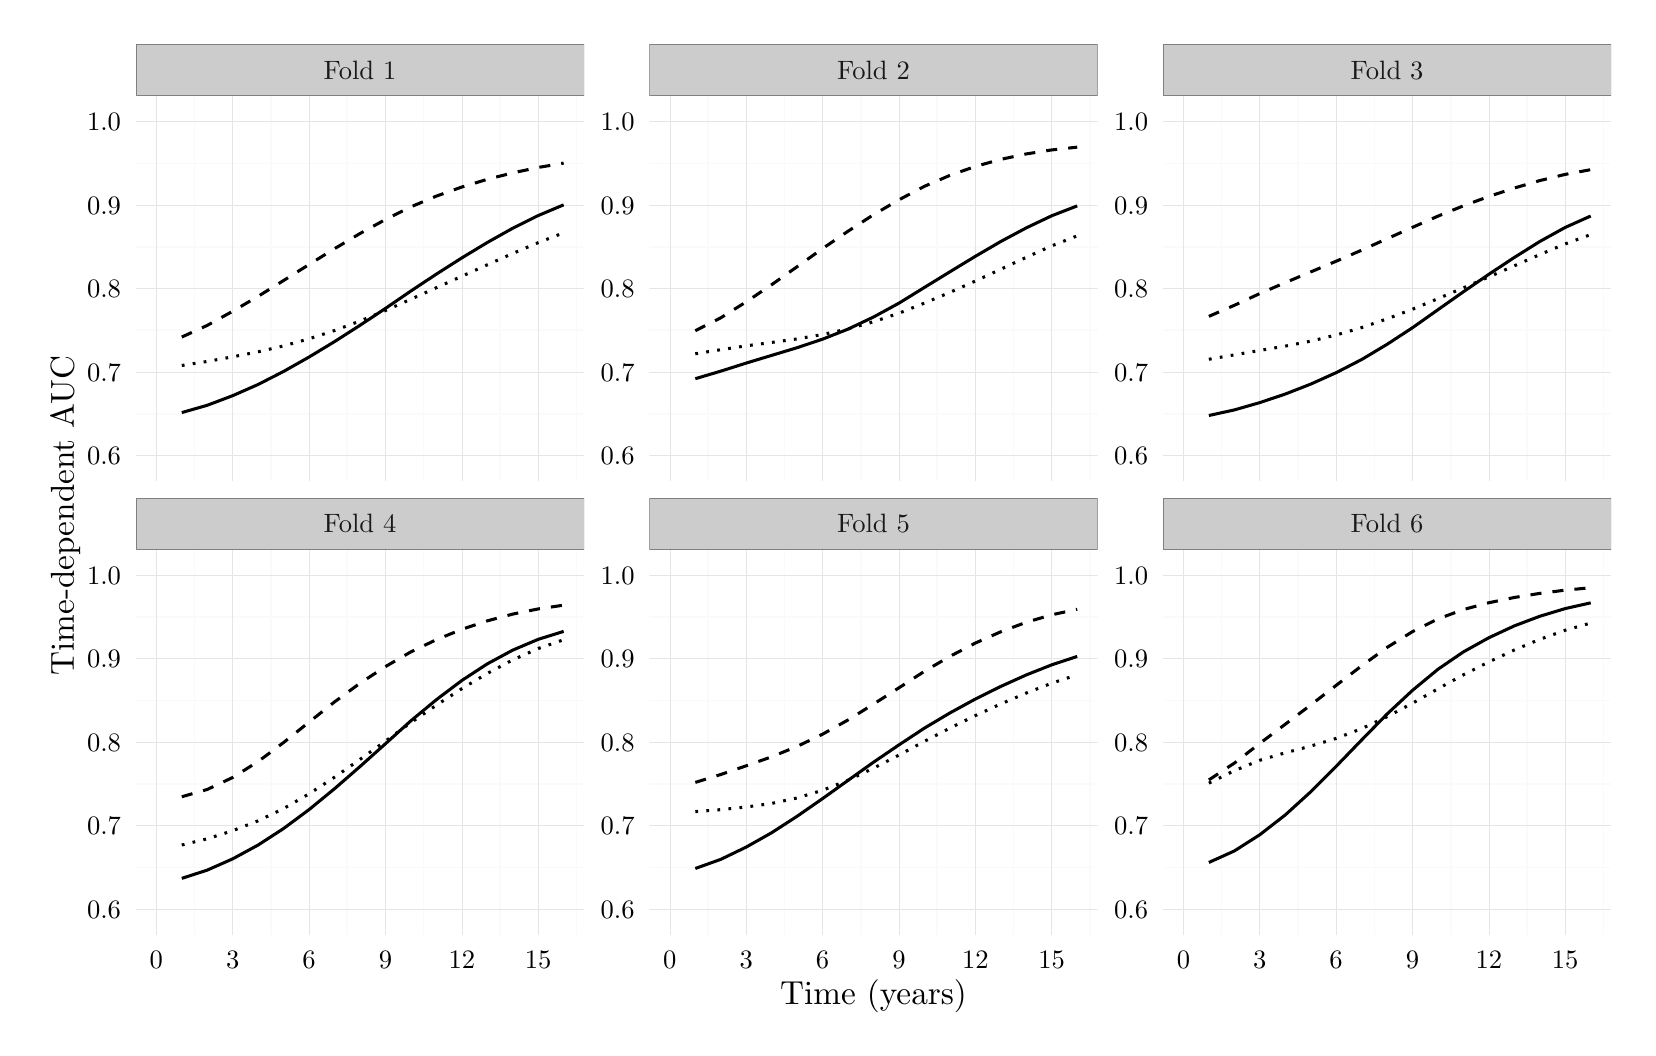
\begin{tikzpicture}[x=1pt,y=1pt]
\definecolor[named]{drawColor}{rgb}{0.00,0.00,0.00}
\definecolor[named]{fillColor}{rgb}{1.00,1.00,1.00}
\fill[color=fillColor,] (0,0) rectangle (578.16,361.35);
\begin{scope}
\path[clip] (  0.00,  0.00) rectangle (578.16,361.35);
\end{scope}
\begin{scope}
\path[clip] (  0.00,  0.00) rectangle (578.16,361.35);
\end{scope}
\begin{scope}
\path[clip] (  0.00,  0.00) rectangle (578.16,361.35);
\end{scope}
\begin{scope}
\path[clip] (  0.00,  0.00) rectangle (578.16,361.35);
\end{scope}
\begin{scope}
\path[clip] (  0.00,  0.00) rectangle (578.16,361.35);
\end{scope}
\begin{scope}
\path[clip] (  0.00,  0.00) rectangle (578.16,361.35);
\end{scope}
\begin{scope}
\path[clip] (  0.00,  0.00) rectangle (578.16,361.35);
\end{scope}
\begin{scope}
\path[clip] (  0.00,  0.00) rectangle (578.16,361.35);
\end{scope}
\begin{scope}
\path[clip] (  0.00,  0.00) rectangle (578.16,361.35);
\end{scope}
\begin{scope}
\path[clip] (  0.00,  0.00) rectangle (578.16,361.35);
\end{scope}
\begin{scope}
\path[clip] (  0.00,  0.00) rectangle (578.16,361.35);
\end{scope}
\begin{scope}
\path[clip] (  0.00,  0.00) rectangle (578.16,361.35);
\end{scope}
\begin{scope}
\path[clip] (  0.00,  0.00) rectangle (578.16,361.35);
\end{scope}
\begin{scope}
\path[clip] (  0.00,  0.00) rectangle (578.16,361.35);
\end{scope}
\begin{scope}
\path[clip] (  0.00,  0.00) rectangle (578.16,361.35);
\end{scope}
\begin{scope}
\path[clip] (  0.00,  0.00) rectangle (578.16,361.35);
\end{scope}
\begin{scope}
\path[clip] (  0.00,  0.00) rectangle (578.16,361.35);
\end{scope}
\begin{scope}
\path[clip] (  0.00,  0.00) rectangle (578.16,361.35);
\end{scope}
\begin{scope}
\path[clip] (  0.00,  0.00) rectangle (578.16,361.35);
\end{scope}
\begin{scope}
\path[clip] (  0.00,  0.00) rectangle (578.16,361.35);
\end{scope}
\begin{scope}
\path[clip] (  0.00,  0.00) rectangle (578.16,361.35);
\end{scope}
\begin{scope}
\path[clip] (  0.00,  0.00) rectangle (578.16,361.35);
\end{scope}
\begin{scope}
\path[clip] (  0.00,  0.00) rectangle (578.16,361.35);
\end{scope}
\begin{scope}
\path[clip] (  0.00,  0.00) rectangle (578.16,361.35);
\end{scope}
\begin{scope}
\path[clip] (  0.00,  0.00) rectangle (578.16,361.35);
\end{scope}
\begin{scope}
\path[clip] (  0.00,  0.00) rectangle (578.16,361.35);
\end{scope}
\begin{scope}
\path[clip] (  0.00,  0.00) rectangle (578.16,361.35);
\end{scope}
\begin{scope}
\path[clip] (  0.00,  0.00) rectangle (578.16,361.35);
\definecolor[named]{drawColor}{rgb}{1.00,1.00,1.00}
\definecolor[named]{fillColor}{rgb}{1.00,1.00,1.00}

\draw[color=drawColor,line width= 0.6pt,line cap=round,line join=round,fill=fillColor,] (  0.00,  0.00) rectangle (578.16,361.35);
\end{scope}
\begin{scope}
\path[clip] (  0.00,  0.00) rectangle (578.16,361.35);
\end{scope}
\begin{scope}
\path[clip] ( 39.13,197.41) rectangle (201.03,336.74);
\definecolor[named]{fillColor}{rgb}{1.00,1.00,1.00}

\draw[fill=fillColor,draw opacity=0.00,] ( 39.13,197.41) rectangle (201.03,336.74);
\definecolor[named]{drawColor}{rgb}{0.98,0.98,0.98}

\draw[color=drawColor,line width= 0.6pt,line join=round,fill opacity=0.00,] ( 39.13,221.84) --
	(201.03,221.84);

\draw[color=drawColor,line width= 0.6pt,line join=round,fill opacity=0.00,] ( 39.13,252.00) --
	(201.03,252.00);

\draw[color=drawColor,line width= 0.6pt,line join=round,fill opacity=0.00,] ( 39.13,282.15) --
	(201.03,282.15);

\draw[color=drawColor,line width= 0.6pt,line join=round,fill opacity=0.00,] ( 39.13,312.31) --
	(201.03,312.31);

\draw[color=drawColor,line width= 0.6pt,line join=round,fill opacity=0.00,] ( 60.29,197.41) --
	( 60.29,336.74);

\draw[color=drawColor,line width= 0.6pt,line join=round,fill opacity=0.00,] ( 87.88,197.41) --
	( 87.88,336.74);

\draw[color=drawColor,line width= 0.6pt,line join=round,fill opacity=0.00,] (115.48,197.41) --
	(115.48,336.74);

\draw[color=drawColor,line width= 0.6pt,line join=round,fill opacity=0.00,] (143.08,197.41) --
	(143.08,336.74);

\draw[color=drawColor,line width= 0.6pt,line join=round,fill opacity=0.00,] (170.67,197.41) --
	(170.67,336.74);

\draw[color=drawColor,line width= 0.6pt,line join=round,fill opacity=0.00,] (198.27,197.41) --
	(198.27,336.74);
\definecolor[named]{drawColor}{rgb}{0.90,0.90,0.90}

\draw[color=drawColor,line width= 0.2pt,line join=round,fill opacity=0.00,] ( 39.13,206.76) --
	(201.03,206.76);

\draw[color=drawColor,line width= 0.2pt,line join=round,fill opacity=0.00,] ( 39.13,236.92) --
	(201.03,236.92);

\draw[color=drawColor,line width= 0.2pt,line join=round,fill opacity=0.00,] ( 39.13,267.08) --
	(201.03,267.08);

\draw[color=drawColor,line width= 0.2pt,line join=round,fill opacity=0.00,] ( 39.13,297.23) --
	(201.03,297.23);

\draw[color=drawColor,line width= 0.2pt,line join=round,fill opacity=0.00,] ( 39.13,327.39) --
	(201.03,327.39);

\draw[color=drawColor,line width= 0.2pt,line join=round,fill opacity=0.00,] ( 46.49,197.41) --
	( 46.49,336.74);

\draw[color=drawColor,line width= 0.2pt,line join=round,fill opacity=0.00,] ( 74.08,197.41) --
	( 74.08,336.74);

\draw[color=drawColor,line width= 0.2pt,line join=round,fill opacity=0.00,] (101.68,197.41) --
	(101.68,336.74);

\draw[color=drawColor,line width= 0.2pt,line join=round,fill opacity=0.00,] (129.28,197.41) --
	(129.28,336.74);

\draw[color=drawColor,line width= 0.2pt,line join=round,fill opacity=0.00,] (156.87,197.41) --
	(156.87,336.74);

\draw[color=drawColor,line width= 0.2pt,line join=round,fill opacity=0.00,] (184.47,197.41) --
	(184.47,336.74);
\definecolor[named]{drawColor}{rgb}{0.00,0.00,0.00}
\definecolor[named]{fillColor}{rgb}{0.00,0.00,0.00}

\draw[color=drawColor,line width= 1.1pt,line join=round,] ( 55.69,222.26) --
	( 64.89,224.90) --
	( 74.08,228.37) --
	( 83.28,232.42) --
	( 92.48,237.13) --
	(101.68,242.33) --
	(110.88,247.90) --
	(120.08,253.79) --
	(129.28,259.90) --
	(138.48,266.20) --
	(147.68,272.29) --
	(156.87,278.15) --
	(166.07,283.71) --
	(175.27,288.87) --
	(184.47,293.45) --
	(193.67,297.33);

\draw[color=drawColor,line width= 1.1pt,dash pattern=on 1pt off 3pt ,line join=round,] ( 55.69,239.28) --
	( 64.89,240.74) --
	( 74.08,242.41) --
	( 83.28,244.22) --
	( 92.48,246.36) --
	(101.68,248.91) --
	(110.88,251.91) --
	(120.08,255.34) --
	(129.28,259.13) --
	(138.48,263.24) --
	(147.68,267.37) --
	(156.87,271.52) --
	(166.07,275.66) --
	(175.27,279.76) --
	(184.47,283.66) --
	(193.67,287.22);

\draw[color=drawColor,line width= 1.1pt,dash pattern=on 4pt off 4pt ,line join=round,] ( 55.69,249.56) --
	( 64.89,253.77) --
	( 74.08,258.88) --
	( 83.28,264.27) --
	( 92.48,269.99) --
	(101.68,275.77) --
	(110.88,281.48) --
	(120.08,286.96) --
	(129.28,292.02) --
	(138.48,296.61) --
	(147.68,300.48) --
	(156.87,303.76) --
	(166.07,306.54) --
	(175.27,308.88) --
	(184.47,310.83) --
	(193.67,312.40);
\end{scope}
\begin{scope}
\path[clip] (  0.00,  0.00) rectangle (578.16,361.35);
\end{scope}
\begin{scope}
\path[clip] (224.69,197.41) rectangle (386.59,336.74);
\definecolor[named]{fillColor}{rgb}{1.00,1.00,1.00}

\draw[fill=fillColor,draw opacity=0.00,] (224.69,197.41) rectangle (386.59,336.74);
\definecolor[named]{drawColor}{rgb}{0.98,0.98,0.98}

\draw[color=drawColor,line width= 0.6pt,line join=round,fill opacity=0.00,] (224.69,221.84) --
	(386.59,221.84);

\draw[color=drawColor,line width= 0.6pt,line join=round,fill opacity=0.00,] (224.69,252.00) --
	(386.59,252.00);

\draw[color=drawColor,line width= 0.6pt,line join=round,fill opacity=0.00,] (224.69,282.15) --
	(386.59,282.15);

\draw[color=drawColor,line width= 0.6pt,line join=round,fill opacity=0.00,] (224.69,312.31) --
	(386.59,312.31);

\draw[color=drawColor,line width= 0.6pt,line join=round,fill opacity=0.00,] (245.85,197.41) --
	(245.85,336.74);

\draw[color=drawColor,line width= 0.6pt,line join=round,fill opacity=0.00,] (273.45,197.41) --
	(273.45,336.74);

\draw[color=drawColor,line width= 0.6pt,line join=round,fill opacity=0.00,] (301.04,197.41) --
	(301.04,336.74);

\draw[color=drawColor,line width= 0.6pt,line join=round,fill opacity=0.00,] (328.64,197.41) --
	(328.64,336.74);

\draw[color=drawColor,line width= 0.6pt,line join=round,fill opacity=0.00,] (356.24,197.41) --
	(356.24,336.74);

\draw[color=drawColor,line width= 0.6pt,line join=round,fill opacity=0.00,] (383.84,197.41) --
	(383.84,336.74);
\definecolor[named]{drawColor}{rgb}{0.90,0.90,0.90}

\draw[color=drawColor,line width= 0.2pt,line join=round,fill opacity=0.00,] (224.69,206.76) --
	(386.59,206.76);

\draw[color=drawColor,line width= 0.2pt,line join=round,fill opacity=0.00,] (224.69,236.92) --
	(386.59,236.92);

\draw[color=drawColor,line width= 0.2pt,line join=round,fill opacity=0.00,] (224.69,267.08) --
	(386.59,267.08);

\draw[color=drawColor,line width= 0.2pt,line join=round,fill opacity=0.00,] (224.69,297.23) --
	(386.59,297.23);

\draw[color=drawColor,line width= 0.2pt,line join=round,fill opacity=0.00,] (224.69,327.39) --
	(386.59,327.39);

\draw[color=drawColor,line width= 0.2pt,line join=round,fill opacity=0.00,] (232.05,197.41) --
	(232.05,336.74);

\draw[color=drawColor,line width= 0.2pt,line join=round,fill opacity=0.00,] (259.65,197.41) --
	(259.65,336.74);

\draw[color=drawColor,line width= 0.2pt,line join=round,fill opacity=0.00,] (287.25,197.41) --
	(287.25,336.74);

\draw[color=drawColor,line width= 0.2pt,line join=round,fill opacity=0.00,] (314.84,197.41) --
	(314.84,336.74);

\draw[color=drawColor,line width= 0.2pt,line join=round,fill opacity=0.00,] (342.44,197.41) --
	(342.44,336.74);

\draw[color=drawColor,line width= 0.2pt,line join=round,fill opacity=0.00,] (370.04,197.41) --
	(370.04,336.74);
\definecolor[named]{drawColor}{rgb}{0.00,0.00,0.00}
\definecolor[named]{fillColor}{rgb}{0.00,0.00,0.00}

\draw[color=drawColor,line width= 1.1pt,line join=round,] (241.25,234.50) --
	(250.45,237.23) --
	(259.65,240.15) --
	(268.85,242.93) --
	(278.05,245.71) --
	(287.25,248.80) --
	(296.45,252.42) --
	(305.64,256.79) --
	(314.84,261.80) --
	(324.04,267.48) --
	(333.24,273.13) --
	(342.44,278.72) --
	(351.64,284.09) --
	(360.84,289.00) --
	(370.04,293.38) --
	(379.24,296.94);

\draw[color=drawColor,line width= 1.1pt,dash pattern=on 1pt off 3pt ,line join=round,] (241.25,243.51) --
	(250.45,244.98) --
	(259.65,246.38) --
	(268.85,247.61) --
	(278.05,248.89) --
	(287.25,250.47) --
	(296.45,252.50) --
	(305.64,255.08) --
	(314.84,258.17) --
	(324.04,261.82) --
	(333.24,265.68) --
	(342.44,269.79) --
	(351.64,274.07) --
	(360.84,278.36) --
	(370.04,282.51) --
	(379.24,286.11);

\draw[color=drawColor,line width= 1.1pt,dash pattern=on 4pt off 4pt ,line join=round,] (241.25,251.85) --
	(250.45,256.51) --
	(259.65,262.28) --
	(268.85,268.48) --
	(278.05,274.98) --
	(287.25,281.54) --
	(296.45,287.81) --
	(305.64,293.76) --
	(314.84,299.15) --
	(324.04,304.02) --
	(333.24,307.97) --
	(342.44,311.20) --
	(351.64,313.77) --
	(360.84,315.72) --
	(370.04,317.17) --
	(379.24,318.17);
\end{scope}
\begin{scope}
\path[clip] (  0.00,  0.00) rectangle (578.16,361.35);
\end{scope}
\begin{scope}
\path[clip] (410.26,197.41) rectangle (572.16,336.74);
\definecolor[named]{fillColor}{rgb}{1.00,1.00,1.00}

\draw[fill=fillColor,draw opacity=0.00,] (410.26,197.41) rectangle (572.16,336.74);
\definecolor[named]{drawColor}{rgb}{0.98,0.98,0.98}

\draw[color=drawColor,line width= 0.6pt,line join=round,fill opacity=0.00,] (410.26,221.84) --
	(572.16,221.84);

\draw[color=drawColor,line width= 0.6pt,line join=round,fill opacity=0.00,] (410.26,252.00) --
	(572.16,252.00);

\draw[color=drawColor,line width= 0.6pt,line join=round,fill opacity=0.00,] (410.26,282.15) --
	(572.16,282.15);

\draw[color=drawColor,line width= 0.6pt,line join=round,fill opacity=0.00,] (410.26,312.31) --
	(572.16,312.31);

\draw[color=drawColor,line width= 0.6pt,line join=round,fill opacity=0.00,] (431.42,197.41) --
	(431.42,336.74);

\draw[color=drawColor,line width= 0.6pt,line join=round,fill opacity=0.00,] (459.01,197.41) --
	(459.01,336.74);

\draw[color=drawColor,line width= 0.6pt,line join=round,fill opacity=0.00,] (486.61,197.41) --
	(486.61,336.74);

\draw[color=drawColor,line width= 0.6pt,line join=round,fill opacity=0.00,] (514.21,197.41) --
	(514.21,336.74);

\draw[color=drawColor,line width= 0.6pt,line join=round,fill opacity=0.00,] (541.80,197.41) --
	(541.80,336.74);

\draw[color=drawColor,line width= 0.6pt,line join=round,fill opacity=0.00,] (569.40,197.41) --
	(569.40,336.74);
\definecolor[named]{drawColor}{rgb}{0.90,0.90,0.90}

\draw[color=drawColor,line width= 0.2pt,line join=round,fill opacity=0.00,] (410.26,206.76) --
	(572.16,206.76);

\draw[color=drawColor,line width= 0.2pt,line join=round,fill opacity=0.00,] (410.26,236.92) --
	(572.16,236.92);

\draw[color=drawColor,line width= 0.2pt,line join=round,fill opacity=0.00,] (410.26,267.08) --
	(572.16,267.08);

\draw[color=drawColor,line width= 0.2pt,line join=round,fill opacity=0.00,] (410.26,297.23) --
	(572.16,297.23);

\draw[color=drawColor,line width= 0.2pt,line join=round,fill opacity=0.00,] (410.26,327.39) --
	(572.16,327.39);

\draw[color=drawColor,line width= 0.2pt,line join=round,fill opacity=0.00,] (417.62,197.41) --
	(417.62,336.74);

\draw[color=drawColor,line width= 0.2pt,line join=round,fill opacity=0.00,] (445.21,197.41) --
	(445.21,336.74);

\draw[color=drawColor,line width= 0.2pt,line join=round,fill opacity=0.00,] (472.81,197.41) --
	(472.81,336.74);

\draw[color=drawColor,line width= 0.2pt,line join=round,fill opacity=0.00,] (500.41,197.41) --
	(500.41,336.74);

\draw[color=drawColor,line width= 0.2pt,line join=round,fill opacity=0.00,] (528.01,197.41) --
	(528.01,336.74);

\draw[color=drawColor,line width= 0.2pt,line join=round,fill opacity=0.00,] (555.60,197.41) --
	(555.60,336.74);
\definecolor[named]{drawColor}{rgb}{0.00,0.00,0.00}
\definecolor[named]{fillColor}{rgb}{0.00,0.00,0.00}

\draw[color=drawColor,line width= 1.1pt,line join=round,] (426.82,221.20) --
	(436.02,223.22) --
	(445.21,225.86) --
	(454.41,228.95) --
	(463.61,232.54) --
	(472.81,236.68) --
	(482.01,241.42) --
	(491.21,246.92) --
	(500.41,252.93) --
	(509.61,259.44) --
	(518.81,265.92) --
	(528.01,272.24) --
	(537.20,278.32) --
	(546.40,284.08) --
	(555.60,289.17) --
	(564.80,293.29);

\draw[color=drawColor,line width= 1.1pt,dash pattern=on 1pt off 3pt ,line join=round,] (426.82,241.53) --
	(436.02,243.12) --
	(445.21,244.71) --
	(454.41,246.27) --
	(463.61,248.07) --
	(472.81,250.29) --
	(482.01,252.97) --
	(491.21,256.13) --
	(500.41,259.61) --
	(509.61,263.44) --
	(518.81,267.34) --
	(528.01,271.29) --
	(537.20,275.30) --
	(546.40,279.35) --
	(555.60,283.21) --
	(564.80,286.58);

\draw[color=drawColor,line width= 1.1pt,dash pattern=on 4pt off 4pt ,line join=round,] (426.82,257.03) --
	(436.02,261.02) --
	(445.21,265.26) --
	(454.41,269.21) --
	(463.61,273.08) --
	(472.81,276.95) --
	(482.01,280.94) --
	(491.21,285.09) --
	(500.41,289.19) --
	(509.61,293.25) --
	(518.81,296.98) --
	(528.01,300.36) --
	(537.20,303.40) --
	(546.40,306.09) --
	(555.60,308.33) --
	(564.80,310.04);
\end{scope}
\begin{scope}
\path[clip] (  0.00,  0.00) rectangle (578.16,361.35);
\end{scope}
\begin{scope}
\path[clip] ( 39.13, 33.48) rectangle (201.03,172.80);
\definecolor[named]{fillColor}{rgb}{1.00,1.00,1.00}

\draw[fill=fillColor,draw opacity=0.00,] ( 39.13, 33.48) rectangle (201.03,172.80);
\definecolor[named]{drawColor}{rgb}{0.98,0.98,0.98}

\draw[color=drawColor,line width= 0.6pt,line join=round,fill opacity=0.00,] ( 39.13, 57.90) --
	(201.03, 57.90);

\draw[color=drawColor,line width= 0.6pt,line join=round,fill opacity=0.00,] ( 39.13, 88.06) --
	(201.03, 88.06);

\draw[color=drawColor,line width= 0.6pt,line join=round,fill opacity=0.00,] ( 39.13,118.22) --
	(201.03,118.22);

\draw[color=drawColor,line width= 0.6pt,line join=round,fill opacity=0.00,] ( 39.13,148.37) --
	(201.03,148.37);

\draw[color=drawColor,line width= 0.6pt,line join=round,fill opacity=0.00,] ( 60.29, 33.48) --
	( 60.29,172.80);

\draw[color=drawColor,line width= 0.6pt,line join=round,fill opacity=0.00,] ( 87.88, 33.48) --
	( 87.88,172.80);

\draw[color=drawColor,line width= 0.6pt,line join=round,fill opacity=0.00,] (115.48, 33.48) --
	(115.48,172.80);

\draw[color=drawColor,line width= 0.6pt,line join=round,fill opacity=0.00,] (143.08, 33.48) --
	(143.08,172.80);

\draw[color=drawColor,line width= 0.6pt,line join=round,fill opacity=0.00,] (170.67, 33.48) --
	(170.67,172.80);

\draw[color=drawColor,line width= 0.6pt,line join=round,fill opacity=0.00,] (198.27, 33.48) --
	(198.27,172.80);
\definecolor[named]{drawColor}{rgb}{0.90,0.90,0.90}

\draw[color=drawColor,line width= 0.2pt,line join=round,fill opacity=0.00,] ( 39.13, 42.83) --
	(201.03, 42.83);

\draw[color=drawColor,line width= 0.2pt,line join=round,fill opacity=0.00,] ( 39.13, 72.98) --
	(201.03, 72.98);

\draw[color=drawColor,line width= 0.2pt,line join=round,fill opacity=0.00,] ( 39.13,103.14) --
	(201.03,103.14);

\draw[color=drawColor,line width= 0.2pt,line join=round,fill opacity=0.00,] ( 39.13,133.30) --
	(201.03,133.30);

\draw[color=drawColor,line width= 0.2pt,line join=round,fill opacity=0.00,] ( 39.13,163.45) --
	(201.03,163.45);

\draw[color=drawColor,line width= 0.2pt,line join=round,fill opacity=0.00,] ( 46.49, 33.48) --
	( 46.49,172.80);

\draw[color=drawColor,line width= 0.2pt,line join=round,fill opacity=0.00,] ( 74.08, 33.48) --
	( 74.08,172.80);

\draw[color=drawColor,line width= 0.2pt,line join=round,fill opacity=0.00,] (101.68, 33.48) --
	(101.68,172.80);

\draw[color=drawColor,line width= 0.2pt,line join=round,fill opacity=0.00,] (129.28, 33.48) --
	(129.28,172.80);

\draw[color=drawColor,line width= 0.2pt,line join=round,fill opacity=0.00,] (156.87, 33.48) --
	(156.87,172.80);

\draw[color=drawColor,line width= 0.2pt,line join=round,fill opacity=0.00,] (184.47, 33.48) --
	(184.47,172.80);
\definecolor[named]{drawColor}{rgb}{0.00,0.00,0.00}
\definecolor[named]{fillColor}{rgb}{0.00,0.00,0.00}

\draw[color=drawColor,line width= 1.1pt,line join=round,] ( 55.69, 53.95) --
	( 64.89, 56.93) --
	( 74.08, 61.00) --
	( 83.28, 66.00) --
	( 92.48, 71.97) --
	(101.68, 78.80) --
	(110.88, 86.34) --
	(120.08, 94.35) --
	(129.28,102.59) --
	(138.48,110.90) --
	(147.68,118.51) --
	(156.87,125.45) --
	(166.07,131.45) --
	(175.27,136.42) --
	(184.47,140.32) --
	(193.67,143.19);

\draw[color=drawColor,line width= 1.1pt,dash pattern=on 1pt off 3pt ,line join=round,] ( 55.69, 66.01) --
	( 64.89, 68.25) --
	( 74.08, 71.17) --
	( 83.28, 74.75) --
	( 92.48, 79.18) --
	(101.68, 84.49) --
	(110.88, 90.50) --
	(120.08, 96.93) --
	(129.28,103.54) --
	(138.48,110.25) --
	(147.68,116.52) --
	(156.87,122.50) --
	(166.07,127.99) --
	(175.27,132.89) --
	(184.47,137.00) --
	(193.67,140.18);

\draw[color=drawColor,line width= 1.1pt,dash pattern=on 4pt off 4pt ,line join=round,] ( 55.69, 83.44) --
	( 64.89, 86.08) --
	( 74.08, 90.40) --
	( 83.28, 96.17) --
	( 92.48,103.04) --
	(101.68,110.41) --
	(110.88,117.71) --
	(120.08,124.46) --
	(129.28,130.47) --
	(138.48,135.80) --
	(147.68,140.20) --
	(156.87,143.94) --
	(166.07,147.00) --
	(175.27,149.44) --
	(184.47,151.31) --
	(193.67,152.67);
\end{scope}
\begin{scope}
\path[clip] (  0.00,  0.00) rectangle (578.16,361.35);
\end{scope}
\begin{scope}
\path[clip] (224.69, 33.48) rectangle (386.59,172.80);
\definecolor[named]{fillColor}{rgb}{1.00,1.00,1.00}

\draw[fill=fillColor,draw opacity=0.00,] (224.69, 33.48) rectangle (386.59,172.80);
\definecolor[named]{drawColor}{rgb}{0.98,0.98,0.98}

\draw[color=drawColor,line width= 0.6pt,line join=round,fill opacity=0.00,] (224.69, 57.90) --
	(386.59, 57.90);

\draw[color=drawColor,line width= 0.6pt,line join=round,fill opacity=0.00,] (224.69, 88.06) --
	(386.59, 88.06);

\draw[color=drawColor,line width= 0.6pt,line join=round,fill opacity=0.00,] (224.69,118.22) --
	(386.59,118.22);

\draw[color=drawColor,line width= 0.6pt,line join=round,fill opacity=0.00,] (224.69,148.37) --
	(386.59,148.37);

\draw[color=drawColor,line width= 0.6pt,line join=round,fill opacity=0.00,] (245.85, 33.48) --
	(245.85,172.80);

\draw[color=drawColor,line width= 0.6pt,line join=round,fill opacity=0.00,] (273.45, 33.48) --
	(273.45,172.80);

\draw[color=drawColor,line width= 0.6pt,line join=round,fill opacity=0.00,] (301.04, 33.48) --
	(301.04,172.80);

\draw[color=drawColor,line width= 0.6pt,line join=round,fill opacity=0.00,] (328.64, 33.48) --
	(328.64,172.80);

\draw[color=drawColor,line width= 0.6pt,line join=round,fill opacity=0.00,] (356.24, 33.48) --
	(356.24,172.80);

\draw[color=drawColor,line width= 0.6pt,line join=round,fill opacity=0.00,] (383.84, 33.48) --
	(383.84,172.80);
\definecolor[named]{drawColor}{rgb}{0.90,0.90,0.90}

\draw[color=drawColor,line width= 0.2pt,line join=round,fill opacity=0.00,] (224.69, 42.83) --
	(386.59, 42.83);

\draw[color=drawColor,line width= 0.2pt,line join=round,fill opacity=0.00,] (224.69, 72.98) --
	(386.59, 72.98);

\draw[color=drawColor,line width= 0.2pt,line join=round,fill opacity=0.00,] (224.69,103.14) --
	(386.59,103.14);

\draw[color=drawColor,line width= 0.2pt,line join=round,fill opacity=0.00,] (224.69,133.30) --
	(386.59,133.30);

\draw[color=drawColor,line width= 0.2pt,line join=round,fill opacity=0.00,] (224.69,163.45) --
	(386.59,163.45);

\draw[color=drawColor,line width= 0.2pt,line join=round,fill opacity=0.00,] (232.05, 33.48) --
	(232.05,172.80);

\draw[color=drawColor,line width= 0.2pt,line join=round,fill opacity=0.00,] (259.65, 33.48) --
	(259.65,172.80);

\draw[color=drawColor,line width= 0.2pt,line join=round,fill opacity=0.00,] (287.25, 33.48) --
	(287.25,172.80);

\draw[color=drawColor,line width= 0.2pt,line join=round,fill opacity=0.00,] (314.84, 33.48) --
	(314.84,172.80);

\draw[color=drawColor,line width= 0.2pt,line join=round,fill opacity=0.00,] (342.44, 33.48) --
	(342.44,172.80);

\draw[color=drawColor,line width= 0.2pt,line join=round,fill opacity=0.00,] (370.04, 33.48) --
	(370.04,172.80);
\definecolor[named]{drawColor}{rgb}{0.00,0.00,0.00}
\definecolor[named]{fillColor}{rgb}{0.00,0.00,0.00}

\draw[color=drawColor,line width= 1.1pt,line join=round,] (241.25, 57.52) --
	(250.45, 60.82) --
	(259.65, 65.26) --
	(268.85, 70.45) --
	(278.05, 76.40) --
	(287.25, 82.79) --
	(296.45, 89.37) --
	(305.64, 95.92) --
	(314.84,102.18) --
	(324.04,108.24) --
	(333.24,113.72) --
	(342.44,118.75) --
	(351.64,123.31) --
	(360.84,127.46) --
	(370.04,131.11) --
	(379.24,134.14);

\draw[color=drawColor,line width= 1.1pt,dash pattern=on 1pt off 3pt ,line join=round,] (241.25, 78.07) --
	(250.45, 78.79) --
	(259.65, 79.74) --
	(268.85, 81.03) --
	(278.05, 83.00) --
	(287.25, 85.79) --
	(296.45, 89.43) --
	(305.64, 93.76) --
	(314.84, 98.48) --
	(324.04,103.47) --
	(333.24,108.24) --
	(342.44,112.77) --
	(351.64,116.98) --
	(360.84,120.91) --
	(370.04,124.47) --
	(379.24,127.51);

\draw[color=drawColor,line width= 1.1pt,dash pattern=on 4pt off 4pt ,line join=round,] (241.25, 88.63) --
	(250.45, 91.48) --
	(259.65, 94.63) --
	(268.85, 97.88) --
	(278.05,101.64) --
	(287.25,106.06) --
	(296.45,111.20) --
	(305.64,116.92) --
	(314.84,122.81) --
	(324.04,128.77) --
	(333.24,134.17) --
	(342.44,138.97) --
	(351.64,143.06) --
	(360.84,146.49) --
	(370.04,149.19) --
	(379.24,151.18);
\end{scope}
\begin{scope}
\path[clip] (  0.00,  0.00) rectangle (578.16,361.35);
\end{scope}
\begin{scope}
\path[clip] (410.26, 33.48) rectangle (572.16,172.80);
\definecolor[named]{fillColor}{rgb}{1.00,1.00,1.00}

\draw[fill=fillColor,draw opacity=0.00,] (410.26, 33.48) rectangle (572.16,172.80);
\definecolor[named]{drawColor}{rgb}{0.98,0.98,0.98}

\draw[color=drawColor,line width= 0.6pt,line join=round,fill opacity=0.00,] (410.26, 57.90) --
	(572.16, 57.90);

\draw[color=drawColor,line width= 0.6pt,line join=round,fill opacity=0.00,] (410.26, 88.06) --
	(572.16, 88.06);

\draw[color=drawColor,line width= 0.6pt,line join=round,fill opacity=0.00,] (410.26,118.22) --
	(572.16,118.22);

\draw[color=drawColor,line width= 0.6pt,line join=round,fill opacity=0.00,] (410.26,148.37) --
	(572.16,148.37);

\draw[color=drawColor,line width= 0.6pt,line join=round,fill opacity=0.00,] (431.42, 33.48) --
	(431.42,172.80);

\draw[color=drawColor,line width= 0.6pt,line join=round,fill opacity=0.00,] (459.01, 33.48) --
	(459.01,172.80);

\draw[color=drawColor,line width= 0.6pt,line join=round,fill opacity=0.00,] (486.61, 33.48) --
	(486.61,172.80);

\draw[color=drawColor,line width= 0.6pt,line join=round,fill opacity=0.00,] (514.21, 33.48) --
	(514.21,172.80);

\draw[color=drawColor,line width= 0.6pt,line join=round,fill opacity=0.00,] (541.80, 33.48) --
	(541.80,172.80);

\draw[color=drawColor,line width= 0.6pt,line join=round,fill opacity=0.00,] (569.40, 33.48) --
	(569.40,172.80);
\definecolor[named]{drawColor}{rgb}{0.90,0.90,0.90}

\draw[color=drawColor,line width= 0.2pt,line join=round,fill opacity=0.00,] (410.26, 42.83) --
	(572.16, 42.83);

\draw[color=drawColor,line width= 0.2pt,line join=round,fill opacity=0.00,] (410.26, 72.98) --
	(572.16, 72.98);

\draw[color=drawColor,line width= 0.2pt,line join=round,fill opacity=0.00,] (410.26,103.14) --
	(572.16,103.14);

\draw[color=drawColor,line width= 0.2pt,line join=round,fill opacity=0.00,] (410.26,133.30) --
	(572.16,133.30);

\draw[color=drawColor,line width= 0.2pt,line join=round,fill opacity=0.00,] (410.26,163.45) --
	(572.16,163.45);

\draw[color=drawColor,line width= 0.2pt,line join=round,fill opacity=0.00,] (417.62, 33.48) --
	(417.62,172.80);

\draw[color=drawColor,line width= 0.2pt,line join=round,fill opacity=0.00,] (445.21, 33.48) --
	(445.21,172.80);

\draw[color=drawColor,line width= 0.2pt,line join=round,fill opacity=0.00,] (472.81, 33.48) --
	(472.81,172.80);

\draw[color=drawColor,line width= 0.2pt,line join=round,fill opacity=0.00,] (500.41, 33.48) --
	(500.41,172.80);

\draw[color=drawColor,line width= 0.2pt,line join=round,fill opacity=0.00,] (528.01, 33.48) --
	(528.01,172.80);

\draw[color=drawColor,line width= 0.2pt,line join=round,fill opacity=0.00,] (555.60, 33.48) --
	(555.60,172.80);
\definecolor[named]{drawColor}{rgb}{0.00,0.00,0.00}
\definecolor[named]{fillColor}{rgb}{0.00,0.00,0.00}

\draw[color=drawColor,line width= 1.1pt,line join=round,] (426.82, 59.70) --
	(436.02, 63.85) --
	(445.21, 69.71) --
	(454.41, 76.85) --
	(463.61, 85.22) --
	(472.81, 94.43) --
	(482.01,103.94) --
	(491.21,113.33) --
	(500.41,121.90) --
	(509.61,129.51) --
	(518.81,135.80) --
	(528.01,140.91) --
	(537.20,145.19) --
	(546.40,148.66) --
	(555.60,151.44) --
	(564.80,153.51);

\draw[color=drawColor,line width= 1.1pt,dash pattern=on 1pt off 3pt ,line join=round,] (426.82, 88.35) --
	(436.02, 92.86) --
	(445.21, 96.62) --
	(454.41, 99.32) --
	(463.61,101.74) --
	(472.81,104.53) --
	(482.01,108.05) --
	(491.21,112.37) --
	(500.41,117.24) --
	(509.61,122.46) --
	(518.81,127.51) --
	(528.01,132.16) --
	(537.20,136.48) --
	(546.40,140.32) --
	(555.60,143.61) --
	(564.80,146.21);

\draw[color=drawColor,line width= 1.1pt,dash pattern=on 4pt off 4pt ,line join=round,] (426.82, 89.53) --
	(436.02, 95.59) --
	(445.21,102.70) --
	(454.41,109.63) --
	(463.61,116.60) --
	(472.81,123.68) --
	(482.01,130.73) --
	(491.21,137.40) --
	(500.41,143.11) --
	(509.61,147.71) --
	(518.81,151.09) --
	(528.01,153.55) --
	(537.20,155.45) --
	(546.40,156.93) --
	(555.60,158.10) --
	(564.80,158.97);
\end{scope}
\begin{scope}
\path[clip] (  0.00,  0.00) rectangle (578.16,361.35);
\end{scope}
\begin{scope}
\path[clip] (  0.00,  0.00) rectangle (578.16,361.35);
\end{scope}
\begin{scope}
\path[clip] ( 39.13,336.74) rectangle (201.03,355.35);
\definecolor[named]{drawColor}{rgb}{0.50,0.50,0.50}
\definecolor[named]{fillColor}{rgb}{0.80,0.80,0.80}

\draw[color=drawColor,line width= 0.2pt,line cap=round,line join=round,fill=fillColor,] ( 39.13,336.74) rectangle (201.03,355.35);
\definecolor[named]{drawColor}{rgb}{0.10,0.10,0.10}

\node[color=drawColor,anchor=base,inner sep=0pt, outer sep=0pt, scale=  0.96] at (120.08,342.74) {Fold 1%
};
\end{scope}
\begin{scope}
\path[clip] ( 39.13,336.74) rectangle (201.03,355.35);
\end{scope}
\begin{scope}
\path[clip] (  0.00,  0.00) rectangle (578.16,361.35);
\end{scope}
\begin{scope}
\path[clip] (  0.00,  0.00) rectangle (578.16,361.35);
\end{scope}
\begin{scope}
\path[clip] (  0.00,  0.00) rectangle (578.16,361.35);
\end{scope}
\begin{scope}
\path[clip] (224.69,336.74) rectangle (386.59,355.35);
\definecolor[named]{drawColor}{rgb}{0.50,0.50,0.50}
\definecolor[named]{fillColor}{rgb}{0.80,0.80,0.80}

\draw[color=drawColor,line width= 0.2pt,line cap=round,line join=round,fill=fillColor,] (224.69,336.74) rectangle (386.59,355.35);
\definecolor[named]{drawColor}{rgb}{0.10,0.10,0.10}

\node[color=drawColor,anchor=base,inner sep=0pt, outer sep=0pt, scale=  0.96] at (305.64,342.74) {Fold 2%
};
\end{scope}
\begin{scope}
\path[clip] (224.69,336.74) rectangle (386.59,355.35);
\end{scope}
\begin{scope}
\path[clip] (  0.00,  0.00) rectangle (578.16,361.35);
\end{scope}
\begin{scope}
\path[clip] (  0.00,  0.00) rectangle (578.16,361.35);
\end{scope}
\begin{scope}
\path[clip] (  0.00,  0.00) rectangle (578.16,361.35);
\end{scope}
\begin{scope}
\path[clip] (410.26,336.74) rectangle (572.16,355.35);
\definecolor[named]{drawColor}{rgb}{0.50,0.50,0.50}
\definecolor[named]{fillColor}{rgb}{0.80,0.80,0.80}

\draw[color=drawColor,line width= 0.2pt,line cap=round,line join=round,fill=fillColor,] (410.26,336.74) rectangle (572.16,355.35);
\definecolor[named]{drawColor}{rgb}{0.10,0.10,0.10}

\node[color=drawColor,anchor=base,inner sep=0pt, outer sep=0pt, scale=  0.96] at (491.21,342.74) {Fold 3%
};
\end{scope}
\begin{scope}
\path[clip] (410.26,336.74) rectangle (572.16,355.35);
\end{scope}
\begin{scope}
\path[clip] (  0.00,  0.00) rectangle (578.16,361.35);
\end{scope}
\begin{scope}
\path[clip] (  0.00,  0.00) rectangle (578.16,361.35);
\end{scope}
\begin{scope}
\path[clip] (  0.00,  0.00) rectangle (578.16,361.35);
\end{scope}
\begin{scope}
\path[clip] ( 39.13,172.80) rectangle (201.03,191.41);
\definecolor[named]{drawColor}{rgb}{0.50,0.50,0.50}
\definecolor[named]{fillColor}{rgb}{0.80,0.80,0.80}

\draw[color=drawColor,line width= 0.2pt,line cap=round,line join=round,fill=fillColor,] ( 39.13,172.80) rectangle (201.03,191.41);
\definecolor[named]{drawColor}{rgb}{0.10,0.10,0.10}

\node[color=drawColor,anchor=base,inner sep=0pt, outer sep=0pt, scale=  0.96] at (120.08,178.80) {Fold 4%
};
\end{scope}
\begin{scope}
\path[clip] ( 39.13,172.80) rectangle (201.03,191.41);
\end{scope}
\begin{scope}
\path[clip] (  0.00,  0.00) rectangle (578.16,361.35);
\end{scope}
\begin{scope}
\path[clip] (  0.00,  0.00) rectangle (578.16,361.35);
\end{scope}
\begin{scope}
\path[clip] (  0.00,  0.00) rectangle (578.16,361.35);
\end{scope}
\begin{scope}
\path[clip] (224.69,172.80) rectangle (386.59,191.41);
\definecolor[named]{drawColor}{rgb}{0.50,0.50,0.50}
\definecolor[named]{fillColor}{rgb}{0.80,0.80,0.80}

\draw[color=drawColor,line width= 0.2pt,line cap=round,line join=round,fill=fillColor,] (224.69,172.80) rectangle (386.59,191.41);
\definecolor[named]{drawColor}{rgb}{0.10,0.10,0.10}

\node[color=drawColor,anchor=base,inner sep=0pt, outer sep=0pt, scale=  0.96] at (305.64,178.80) {Fold 5%
};
\end{scope}
\begin{scope}
\path[clip] (224.69,172.80) rectangle (386.59,191.41);
\end{scope}
\begin{scope}
\path[clip] (  0.00,  0.00) rectangle (578.16,361.35);
\end{scope}
\begin{scope}
\path[clip] (  0.00,  0.00) rectangle (578.16,361.35);
\end{scope}
\begin{scope}
\path[clip] (  0.00,  0.00) rectangle (578.16,361.35);
\end{scope}
\begin{scope}
\path[clip] (410.26,172.80) rectangle (572.16,191.41);
\definecolor[named]{drawColor}{rgb}{0.50,0.50,0.50}
\definecolor[named]{fillColor}{rgb}{0.80,0.80,0.80}

\draw[color=drawColor,line width= 0.2pt,line cap=round,line join=round,fill=fillColor,] (410.26,172.80) rectangle (572.16,191.41);
\definecolor[named]{drawColor}{rgb}{0.10,0.10,0.10}

\node[color=drawColor,anchor=base,inner sep=0pt, outer sep=0pt, scale=  0.96] at (491.21,178.80) {Fold 6%
};
\end{scope}
\begin{scope}
\path[clip] (410.26,172.80) rectangle (572.16,191.41);
\end{scope}
\begin{scope}
\path[clip] (  0.00,  0.00) rectangle (578.16,361.35);
\end{scope}
\begin{scope}
\path[clip] (  0.00,  0.00) rectangle (578.16,361.35);
\end{scope}
\begin{scope}
\path[clip] (  0.00,  0.00) rectangle (578.16,361.35);
\end{scope}
\begin{scope}
\path[clip] (  0.00,  0.00) rectangle (578.16,361.35);
\end{scope}
\begin{scope}
\path[clip] (  0.00,  0.00) rectangle (578.16,361.35);
\end{scope}
\begin{scope}
\path[clip] (  0.00,  0.00) rectangle (578.16,361.35);
\end{scope}
\begin{scope}
\path[clip] (  0.00,  0.00) rectangle (578.16,361.35);
\definecolor[named]{drawColor}{rgb}{0.00,0.00,0.00}

\node[color=drawColor,anchor=base east,inner sep=0pt, outer sep=0pt, scale=  0.96] at ( 33.73,203.46) {0.6%
};

\node[color=drawColor,anchor=base east,inner sep=0pt, outer sep=0pt, scale=  0.96] at ( 33.73,233.61) {0.7%
};

\node[color=drawColor,anchor=base east,inner sep=0pt, outer sep=0pt, scale=  0.96] at ( 33.73,263.77) {0.8%
};

\node[color=drawColor,anchor=base east,inner sep=0pt, outer sep=0pt, scale=  0.96] at ( 33.73,293.93) {0.9%
};

\node[color=drawColor,anchor=base east,inner sep=0pt, outer sep=0pt, scale=  0.96] at ( 33.73,324.08) {1.0%
};
\end{scope}
\begin{scope}
\path[clip] (  0.00,  0.00) rectangle (578.16,361.35);
\end{scope}
\begin{scope}
\path[clip] (  0.00,  0.00) rectangle (578.16,361.35);
\end{scope}
\begin{scope}
\path[clip] (  0.00,  0.00) rectangle (578.16,361.35);
\end{scope}
\begin{scope}
\path[clip] (  0.00,  0.00) rectangle (578.16,361.35);
\end{scope}
\begin{scope}
\path[clip] (  0.00,  0.00) rectangle (578.16,361.35);
\end{scope}
\begin{scope}
\path[clip] (  0.00,  0.00) rectangle (578.16,361.35);
\end{scope}
\begin{scope}
\path[clip] (  0.00,  0.00) rectangle (578.16,361.35);
\end{scope}
\begin{scope}
\path[clip] (  0.00,  0.00) rectangle (578.16,361.35);
\end{scope}
\begin{scope}
\path[clip] (  0.00,  0.00) rectangle (578.16,361.35);
\end{scope}
\begin{scope}
\path[clip] (  0.00,  0.00) rectangle (578.16,361.35);
\definecolor[named]{drawColor}{rgb}{0.00,0.00,0.00}

\node[color=drawColor,anchor=base east,inner sep=0pt, outer sep=0pt, scale=  0.96] at (219.29,203.46) {0.6%
};

\node[color=drawColor,anchor=base east,inner sep=0pt, outer sep=0pt, scale=  0.96] at (219.29,233.61) {0.7%
};

\node[color=drawColor,anchor=base east,inner sep=0pt, outer sep=0pt, scale=  0.96] at (219.29,263.77) {0.8%
};

\node[color=drawColor,anchor=base east,inner sep=0pt, outer sep=0pt, scale=  0.96] at (219.29,293.93) {0.9%
};

\node[color=drawColor,anchor=base east,inner sep=0pt, outer sep=0pt, scale=  0.96] at (219.29,324.08) {1.0%
};
\end{scope}
\begin{scope}
\path[clip] (  0.00,  0.00) rectangle (578.16,361.35);
\end{scope}
\begin{scope}
\path[clip] (  0.00,  0.00) rectangle (578.16,361.35);
\end{scope}
\begin{scope}
\path[clip] (  0.00,  0.00) rectangle (578.16,361.35);
\end{scope}
\begin{scope}
\path[clip] (  0.00,  0.00) rectangle (578.16,361.35);
\end{scope}
\begin{scope}
\path[clip] (  0.00,  0.00) rectangle (578.16,361.35);
\end{scope}
\begin{scope}
\path[clip] (  0.00,  0.00) rectangle (578.16,361.35);
\end{scope}
\begin{scope}
\path[clip] (  0.00,  0.00) rectangle (578.16,361.35);
\end{scope}
\begin{scope}
\path[clip] (  0.00,  0.00) rectangle (578.16,361.35);
\end{scope}
\begin{scope}
\path[clip] (  0.00,  0.00) rectangle (578.16,361.35);
\end{scope}
\begin{scope}
\path[clip] (  0.00,  0.00) rectangle (578.16,361.35);
\definecolor[named]{drawColor}{rgb}{0.00,0.00,0.00}

\node[color=drawColor,anchor=base east,inner sep=0pt, outer sep=0pt, scale=  0.96] at (404.86,203.46) {0.6%
};

\node[color=drawColor,anchor=base east,inner sep=0pt, outer sep=0pt, scale=  0.96] at (404.86,233.61) {0.7%
};

\node[color=drawColor,anchor=base east,inner sep=0pt, outer sep=0pt, scale=  0.96] at (404.86,263.77) {0.8%
};

\node[color=drawColor,anchor=base east,inner sep=0pt, outer sep=0pt, scale=  0.96] at (404.86,293.93) {0.9%
};

\node[color=drawColor,anchor=base east,inner sep=0pt, outer sep=0pt, scale=  0.96] at (404.86,324.08) {1.0%
};
\end{scope}
\begin{scope}
\path[clip] (  0.00,  0.00) rectangle (578.16,361.35);
\end{scope}
\begin{scope}
\path[clip] (  0.00,  0.00) rectangle (578.16,361.35);
\end{scope}
\begin{scope}
\path[clip] (  0.00,  0.00) rectangle (578.16,361.35);
\end{scope}
\begin{scope}
\path[clip] (  0.00,  0.00) rectangle (578.16,361.35);
\end{scope}
\begin{scope}
\path[clip] (  0.00,  0.00) rectangle (578.16,361.35);
\end{scope}
\begin{scope}
\path[clip] (  0.00,  0.00) rectangle (578.16,361.35);
\end{scope}
\begin{scope}
\path[clip] (  0.00,  0.00) rectangle (578.16,361.35);
\end{scope}
\begin{scope}
\path[clip] (  0.00,  0.00) rectangle (578.16,361.35);
\end{scope}
\begin{scope}
\path[clip] (  0.00,  0.00) rectangle (578.16,361.35);
\end{scope}
\begin{scope}
\path[clip] (  0.00,  0.00) rectangle (578.16,361.35);
\definecolor[named]{drawColor}{rgb}{0.00,0.00,0.00}

\node[color=drawColor,anchor=base east,inner sep=0pt, outer sep=0pt, scale=  0.96] at ( 33.73, 39.52) {0.6%
};

\node[color=drawColor,anchor=base east,inner sep=0pt, outer sep=0pt, scale=  0.96] at ( 33.73, 69.68) {0.7%
};

\node[color=drawColor,anchor=base east,inner sep=0pt, outer sep=0pt, scale=  0.96] at ( 33.73, 99.83) {0.8%
};

\node[color=drawColor,anchor=base east,inner sep=0pt, outer sep=0pt, scale=  0.96] at ( 33.73,129.99) {0.9%
};

\node[color=drawColor,anchor=base east,inner sep=0pt, outer sep=0pt, scale=  0.96] at ( 33.73,160.15) {1.0%
};
\end{scope}
\begin{scope}
\path[clip] (  0.00,  0.00) rectangle (578.16,361.35);
\end{scope}
\begin{scope}
\path[clip] (  0.00,  0.00) rectangle (578.16,361.35);
\end{scope}
\begin{scope}
\path[clip] (  0.00,  0.00) rectangle (578.16,361.35);
\end{scope}
\begin{scope}
\path[clip] (  0.00,  0.00) rectangle (578.16,361.35);
\end{scope}
\begin{scope}
\path[clip] (  0.00,  0.00) rectangle (578.16,361.35);
\end{scope}
\begin{scope}
\path[clip] (  0.00,  0.00) rectangle (578.16,361.35);
\end{scope}
\begin{scope}
\path[clip] (  0.00,  0.00) rectangle (578.16,361.35);
\end{scope}
\begin{scope}
\path[clip] (  0.00,  0.00) rectangle (578.16,361.35);
\end{scope}
\begin{scope}
\path[clip] (  0.00,  0.00) rectangle (578.16,361.35);
\end{scope}
\begin{scope}
\path[clip] (  0.00,  0.00) rectangle (578.16,361.35);
\definecolor[named]{drawColor}{rgb}{0.00,0.00,0.00}

\node[color=drawColor,anchor=base east,inner sep=0pt, outer sep=0pt, scale=  0.96] at (219.29, 39.52) {0.6%
};

\node[color=drawColor,anchor=base east,inner sep=0pt, outer sep=0pt, scale=  0.96] at (219.29, 69.68) {0.7%
};

\node[color=drawColor,anchor=base east,inner sep=0pt, outer sep=0pt, scale=  0.96] at (219.29, 99.83) {0.8%
};

\node[color=drawColor,anchor=base east,inner sep=0pt, outer sep=0pt, scale=  0.96] at (219.29,129.99) {0.9%
};

\node[color=drawColor,anchor=base east,inner sep=0pt, outer sep=0pt, scale=  0.96] at (219.29,160.15) {1.0%
};
\end{scope}
\begin{scope}
\path[clip] (  0.00,  0.00) rectangle (578.16,361.35);
\end{scope}
\begin{scope}
\path[clip] (  0.00,  0.00) rectangle (578.16,361.35);
\end{scope}
\begin{scope}
\path[clip] (  0.00,  0.00) rectangle (578.16,361.35);
\end{scope}
\begin{scope}
\path[clip] (  0.00,  0.00) rectangle (578.16,361.35);
\end{scope}
\begin{scope}
\path[clip] (  0.00,  0.00) rectangle (578.16,361.35);
\end{scope}
\begin{scope}
\path[clip] (  0.00,  0.00) rectangle (578.16,361.35);
\end{scope}
\begin{scope}
\path[clip] (  0.00,  0.00) rectangle (578.16,361.35);
\end{scope}
\begin{scope}
\path[clip] (  0.00,  0.00) rectangle (578.16,361.35);
\end{scope}
\begin{scope}
\path[clip] (  0.00,  0.00) rectangle (578.16,361.35);
\end{scope}
\begin{scope}
\path[clip] (  0.00,  0.00) rectangle (578.16,361.35);
\definecolor[named]{drawColor}{rgb}{0.00,0.00,0.00}

\node[color=drawColor,anchor=base east,inner sep=0pt, outer sep=0pt, scale=  0.96] at (404.86, 39.52) {0.6%
};

\node[color=drawColor,anchor=base east,inner sep=0pt, outer sep=0pt, scale=  0.96] at (404.86, 69.68) {0.7%
};

\node[color=drawColor,anchor=base east,inner sep=0pt, outer sep=0pt, scale=  0.96] at (404.86, 99.83) {0.8%
};

\node[color=drawColor,anchor=base east,inner sep=0pt, outer sep=0pt, scale=  0.96] at (404.86,129.99) {0.9%
};

\node[color=drawColor,anchor=base east,inner sep=0pt, outer sep=0pt, scale=  0.96] at (404.86,160.15) {1.0%
};
\end{scope}
\begin{scope}
\path[clip] (  0.00,  0.00) rectangle (578.16,361.35);
\end{scope}
\begin{scope}
\path[clip] (  0.00,  0.00) rectangle (578.16,361.35);
\end{scope}
\begin{scope}
\path[clip] (  0.00,  0.00) rectangle (578.16,361.35);
\end{scope}
\begin{scope}
\path[clip] (  0.00,  0.00) rectangle (578.16,361.35);
\end{scope}
\begin{scope}
\path[clip] (  0.00,  0.00) rectangle (578.16,361.35);
\end{scope}
\begin{scope}
\path[clip] (  0.00,  0.00) rectangle (578.16,361.35);
\end{scope}
\begin{scope}
\path[clip] (  0.00,  0.00) rectangle (578.16,361.35);
\end{scope}
\begin{scope}
\path[clip] (  0.00,  0.00) rectangle (578.16,361.35);
\end{scope}
\begin{scope}
\path[clip] (  0.00,  0.00) rectangle (578.16,361.35);
\end{scope}
\begin{scope}
\path[clip] (  0.00,  0.00) rectangle (578.16,361.35);
\end{scope}
\begin{scope}
\path[clip] (  0.00,  0.00) rectangle (578.16,361.35);
\end{scope}
\begin{scope}
\path[clip] (  0.00,  0.00) rectangle (578.16,361.35);
\end{scope}
\begin{scope}
\path[clip] (  0.00,  0.00) rectangle (578.16,361.35);
\end{scope}
\begin{scope}
\path[clip] (  0.00,  0.00) rectangle (578.16,361.35);
\end{scope}
\begin{scope}
\path[clip] (  0.00,  0.00) rectangle (578.16,361.35);
\end{scope}
\begin{scope}
\path[clip] (  0.00,  0.00) rectangle (578.16,361.35);
\end{scope}
\begin{scope}
\path[clip] (  0.00,  0.00) rectangle (578.16,361.35);
\end{scope}
\begin{scope}
\path[clip] (  0.00,  0.00) rectangle (578.16,361.35);
\definecolor[named]{drawColor}{rgb}{0.00,0.00,0.00}

\node[color=drawColor,anchor=base,inner sep=0pt, outer sep=0pt, scale=  0.96] at ( 46.49, 21.46) {0%
};

\node[color=drawColor,anchor=base,inner sep=0pt, outer sep=0pt, scale=  0.96] at ( 74.08, 21.46) {3%
};

\node[color=drawColor,anchor=base,inner sep=0pt, outer sep=0pt, scale=  0.96] at (101.68, 21.46) {6%
};

\node[color=drawColor,anchor=base,inner sep=0pt, outer sep=0pt, scale=  0.96] at (129.28, 21.46) {9%
};

\node[color=drawColor,anchor=base,inner sep=0pt, outer sep=0pt, scale=  0.96] at (156.87, 21.46) {12%
};

\node[color=drawColor,anchor=base,inner sep=0pt, outer sep=0pt, scale=  0.96] at (184.47, 21.46) {15%
};
\end{scope}
\begin{scope}
\path[clip] (  0.00,  0.00) rectangle (578.16,361.35);
\end{scope}
\begin{scope}
\path[clip] (  0.00,  0.00) rectangle (578.16,361.35);
\end{scope}
\begin{scope}
\path[clip] (  0.00,  0.00) rectangle (578.16,361.35);
\end{scope}
\begin{scope}
\path[clip] (  0.00,  0.00) rectangle (578.16,361.35);
\end{scope}
\begin{scope}
\path[clip] (  0.00,  0.00) rectangle (578.16,361.35);
\end{scope}
\begin{scope}
\path[clip] (  0.00,  0.00) rectangle (578.16,361.35);
\end{scope}
\begin{scope}
\path[clip] (  0.00,  0.00) rectangle (578.16,361.35);
\end{scope}
\begin{scope}
\path[clip] (  0.00,  0.00) rectangle (578.16,361.35);
\end{scope}
\begin{scope}
\path[clip] (  0.00,  0.00) rectangle (578.16,361.35);
\end{scope}
\begin{scope}
\path[clip] (  0.00,  0.00) rectangle (578.16,361.35);
\definecolor[named]{drawColor}{rgb}{0.00,0.00,0.00}

\node[color=drawColor,anchor=base,inner sep=0pt, outer sep=0pt, scale=  0.96] at (232.05, 21.46) {0%
};

\node[color=drawColor,anchor=base,inner sep=0pt, outer sep=0pt, scale=  0.96] at (259.65, 21.46) {3%
};

\node[color=drawColor,anchor=base,inner sep=0pt, outer sep=0pt, scale=  0.96] at (287.25, 21.46) {6%
};

\node[color=drawColor,anchor=base,inner sep=0pt, outer sep=0pt, scale=  0.96] at (314.84, 21.46) {9%
};

\node[color=drawColor,anchor=base,inner sep=0pt, outer sep=0pt, scale=  0.96] at (342.44, 21.46) {12%
};

\node[color=drawColor,anchor=base,inner sep=0pt, outer sep=0pt, scale=  0.96] at (370.04, 21.46) {15%
};
\end{scope}
\begin{scope}
\path[clip] (  0.00,  0.00) rectangle (578.16,361.35);
\end{scope}
\begin{scope}
\path[clip] (  0.00,  0.00) rectangle (578.16,361.35);
\end{scope}
\begin{scope}
\path[clip] (  0.00,  0.00) rectangle (578.16,361.35);
\end{scope}
\begin{scope}
\path[clip] (  0.00,  0.00) rectangle (578.16,361.35);
\end{scope}
\begin{scope}
\path[clip] (  0.00,  0.00) rectangle (578.16,361.35);
\end{scope}
\begin{scope}
\path[clip] (  0.00,  0.00) rectangle (578.16,361.35);
\end{scope}
\begin{scope}
\path[clip] (  0.00,  0.00) rectangle (578.16,361.35);
\end{scope}
\begin{scope}
\path[clip] (  0.00,  0.00) rectangle (578.16,361.35);
\end{scope}
\begin{scope}
\path[clip] (  0.00,  0.00) rectangle (578.16,361.35);
\end{scope}
\begin{scope}
\path[clip] (  0.00,  0.00) rectangle (578.16,361.35);
\definecolor[named]{drawColor}{rgb}{0.00,0.00,0.00}

\node[color=drawColor,anchor=base,inner sep=0pt, outer sep=0pt, scale=  0.96] at (417.62, 21.46) {0%
};

\node[color=drawColor,anchor=base,inner sep=0pt, outer sep=0pt, scale=  0.96] at (445.21, 21.46) {3%
};

\node[color=drawColor,anchor=base,inner sep=0pt, outer sep=0pt, scale=  0.96] at (472.81, 21.46) {6%
};

\node[color=drawColor,anchor=base,inner sep=0pt, outer sep=0pt, scale=  0.96] at (500.41, 21.46) {9%
};

\node[color=drawColor,anchor=base,inner sep=0pt, outer sep=0pt, scale=  0.96] at (528.01, 21.46) {12%
};

\node[color=drawColor,anchor=base,inner sep=0pt, outer sep=0pt, scale=  0.96] at (555.60, 21.46) {15%
};
\end{scope}
\begin{scope}
\path[clip] (  0.00,  0.00) rectangle (578.16,361.35);
\end{scope}
\begin{scope}
\path[clip] (  0.00,  0.00) rectangle (578.16,361.35);
\end{scope}
\begin{scope}
\path[clip] (  0.00,  0.00) rectangle (578.16,361.35);
\end{scope}
\begin{scope}
\path[clip] (  0.00,  0.00) rectangle (578.16,361.35);
\definecolor[named]{drawColor}{rgb}{0.00,0.00,0.00}

\node[color=drawColor,anchor=base,inner sep=0pt, outer sep=0pt, scale=  1.20] at (305.64,  8.40) {Time (years)%
};
\end{scope}
\begin{scope}
\path[clip] (  0.00,  0.00) rectangle (578.16,361.35);
\end{scope}
\begin{scope}
\path[clip] (  0.00,  0.00) rectangle (578.16,361.35);
\definecolor[named]{drawColor}{rgb}{0.00,0.00,0.00}

\node[rotate= 90.00,color=drawColor,anchor=base,inner sep=0pt, outer sep=0pt, scale=  1.20] at ( 16.66,185.11) {Time-dependent AUC%
};
\end{scope}
\begin{scope}
\path[clip] (  0.00,  0.00) rectangle (578.16,361.35);
\end{scope}
\begin{scope}
\path[clip] (  0.00,  0.00) rectangle (578.16,361.35);
\end{scope}
\begin{scope}
\path[clip] (  0.00,  0.00) rectangle (578.16,361.35);
\end{scope}
\begin{scope}
\path[clip] (  0.00,  0.00) rectangle (578.16,361.35);
\end{scope}
\end{tikzpicture}
}
	\label{fig:auc}
\end{figure}